\documentclass[11pt]{article}
\usepackage{iitbtitle}
\usepackage{caption}
\usepackage{subcaption}
\usepackage{a4wide}
\usepackage{multirow} 
\usepackage{anysize}
\usepackage{iitbcs}
\usepackage{latexsym}
\usepackage{amssymb}
\usepackage{amsmath}
\usepackage{graphicx}
\usepackage{epsfig}
\usepackage{comment}
% \usepackage{psfig}
\usepackage{tabls}
\usepackage{multirow}
\usepackage{tabularx}
\usepackage{url}
\newcolumntype{Y}{>{\centering\arraybackslash}X}
\setlength{\floatsep}{7pt plus 2pt minus 2pt}
\setlength{\textfloatsep}{5pt plus 2pt minus 2pt}
\setlength{\intextsep}{5pt plus 2pt minus 2pt}
\usepackage{color}

\marginsize{2.5cm}{2.5cm}{1cm}{1.5cm}
\def\baselinestretch{1.15}

\newcommand\INPUT{\item[\textbf{Input:}]}
\newcommand\OUTPUT{\item[\textbf{Output:}]}
\providecommand{\norm}[1]{\lVert#1\rVert}
\DeclareGraphicsExtensions{.pdf,.png,.jpg}
\begin{document}


%\baselineskip 20pt
%The definitions
\def\title{Quadcopter Based Applications in Imaging}
\def\what{Third Annual Progress Report}
\def\degree{Doctor of Philosophy}
\def\who{Meghshyam G. Prasad}
\def\roll{124058001}
\def\guide{Prof. Sharat Chandran \\ Prof. Michael Brown}
\titlpage
\def\bsq{\begin{flushright} $\blacksquare$\\ \end{flushright}}
\def\tab{\hspace{5mm}}

\newpage
\section*{Acknowledgements}
I express deep and sincere gratitude to Prof. Sharat Chandran and Prof.
Michael Brown for providing constant direction and guidance. I am also
very much grateful to Prof. David Hsu for giving me access to his lab and
equipments. I am also thankful to Mr. Abhishek Chakrborty and Mr. Ravi Chalasani
for their help in stagnant water detection project.

\begin{flushright}
Meghshyam G. Prasad
\end{flushright}

\pagenumbering{roman}
\newpage
\begin{abstract}
In today's world, digital imaging is being extensively used in almost all
sectors. In some situations, it is quite difficult to take pictures from
handheld camera. Low cost quadcopters such as Parrot's AR Drone may be used in
such scenarios to take photos of an object which is otherwise out of reach of normal
camera. There are two problems involved in it: first to track the given object
and second to take ``good'' pictures of it. In my last APS we discussed 
about the first problem. Here, we will see how to take good pictures and use it for
various applications.

One of the use case where we may use quadcopter for imaging is to
capture a panaroma of big wall (or any such planar object). In such cases, it
will be very tedious and tiring to use hand held camera. Secondly, if there are
vacant spaces on a wall, it is challenging for existing mosaicing techniques as
there will be little to no features to match input images. So, in our work, we
focuses on a method to construct panoramas captured from a quadcopter, that
consists of scenes with significant regions of vacant spaces.

We describe a framework that is able to handle this unique input by
leveraging the availability of the inertial measurement unit (IMU)
data from the quadcopter that is synchronized with the input images.
We use the IMU data for two purposes: first to select images which can
be stitched together. Second, in combination with coarse stereo reconstruction,
we determine appropriate portions of the images to complete the panorama. We
demonstrate the efficacy of our approach on a number of input sequences that
cannot to be mosaiced by existing methods.

After using quadcopter for mosaicing of images, we thought of using it for 
some ``survey'' application. In recent times, there has been a sharp increase
in dengue and malaria, especially in urban areas. One of the major reasons for
this health hazard is the number of locations where one can find stagnant
water. These locations are large breeding ground for fast multiplying
mosquitoes, and other insects. Areas include traditionally uncovered gutters,
and also terraces of high rise buildings, and shades above windows (popularly
known as chhajja)-- areas that are hard to reach and access. We propose the use
of a quadcopter to inspect areas and identify stagnant water patches.  Water
being specular in nature tends to confound traditional image processing
methods. Further the use of a non-traditional camera mounted on a quadcopter
presents new challenges.  We provide methods to get past such hurdles.

\noindent \textbf{Keywords:} Quadcopter, Panoramic Image Stitching, Stagnant Water Detection

\end{abstract}
\newpage
\pagenumbering{arabic}
\tableofcontents

%\begingroup\def\thispagestyle#1{}\def\baselinestretch{1.5}\tableofcontents\endgroup
\newpage

\section{Introduction}

\section{Mosaicing Scenes with Vacant Spaces}

Finding features and using them to align images to construct wide field
of view panoramas is one of the success stories of
computer vision.  Virtually all recent consumer cameras have this
technology embedded.  The success of these methods relies significantly on
finding common features in the images that can be used to established the
 appropriate warps to register the images together.

There are scenes, however, that consist of image content that makes this
challenging.  One situation is when scene patterns and texture are repeated.  
This can make it challenging for matching algorithm to find appropriate matches.
A more serious situation is when a scene area simply
does not contain features.  This sort of situation occurs in a variety
of situations such as paintings in an art exhibition, or posters in an
auditorium.

{\bf Key Idea} We propose to solve the vacant space problem by using
an inexpensive off-the-shelf flying device, such as a quadcopter which
can be assumed to contain an inertial measurement unit (IMU) that has
positional information time synchronized with an input video.  The
proximity relationship that the resultant images have, can be used to
significantly reduce the search space in finding matches.  Further,
the proximity relationship also allows, in principle, to vary the
parameters involved in feature selection. For example, if there is
reason to believe that two images are adjacent horizontally, one can
choose to adjust thresholds in feature matching algorithm to hunt for
otherwise elusive matching pairs.

We note that positions can be also made available in other devices
such as smartphones.  An autonomous programmed quadcopter, however, is
particularly enticing because of its ability to fly to areas that are
accessible to the human eye, but inaccessible for the
human to reach.  Such areas do not lend themselves easily to high
quality images.

\subsection{Related Work}
Panoramic image stitching (alternatively, image mosaicing) is a
well-studied problem in the field of computer vision.  Representative
works include~\cite{Milgram1975}, \cite{Milgram1977}, \cite{Capel},
\cite{Szeliski1997} \cite{Brown07} \cite{Brown03}.  A full discussion
on related works is outside the scope of this report, readers are
referred to~\cite{Szeliski05imagealignment} for an excellent survey.
Given the maturity of this area, there are various freeware as well as
commercial software available for performing image stitching; most
notable are AutoStitch \cite{autostitch}, Microsoft\textsc{\char13}s Image
Compositing Editor \cite{ICE}, and Adobe\textsc{\char13}s Photoshop
\cite{photoshop}.

All of these methods are based on a similar strategy of finding
features in each image, matching these features between images, and
then computing pairwise image warps to align them together.  A global
bundle adjustment is often applied to globally refine the alignment.
All of the aforementioned methods assume the imaged scene is planar or
that the camera has been rotated carefully around its center of
projection to avoid parallax.

Brown et al.~\cite{Brown05} have used a new type of invariant features
located at Harris corners in discrete scale-space and oriented using a
blurred local gradient for stitching. Eden et al.~\cite{Eden} were
able to stitch images with large exposure difference as well as large
scene motion into single HDR quality image without using any
additional camera hardware.

All of the image mosaicing methods work only when there is a
``intersection'' in feature space of images to be stitched. When there
are ``gaps'' (either physical or due to lack of features) between
images to be stitched it is not clear how to perform the stitching. We discuss
how to use the available IMU data that accompanies our input images to help
overcome these problems.

\subsection{Methodology}
Our goal is to compute a panorama of a scene lying on
planar surface that has regions of vacant spaces.  A schematic for
this problem is shown in Figure~\ref{fig:schematic}.

\begin{figure}[h!]
  \centering
  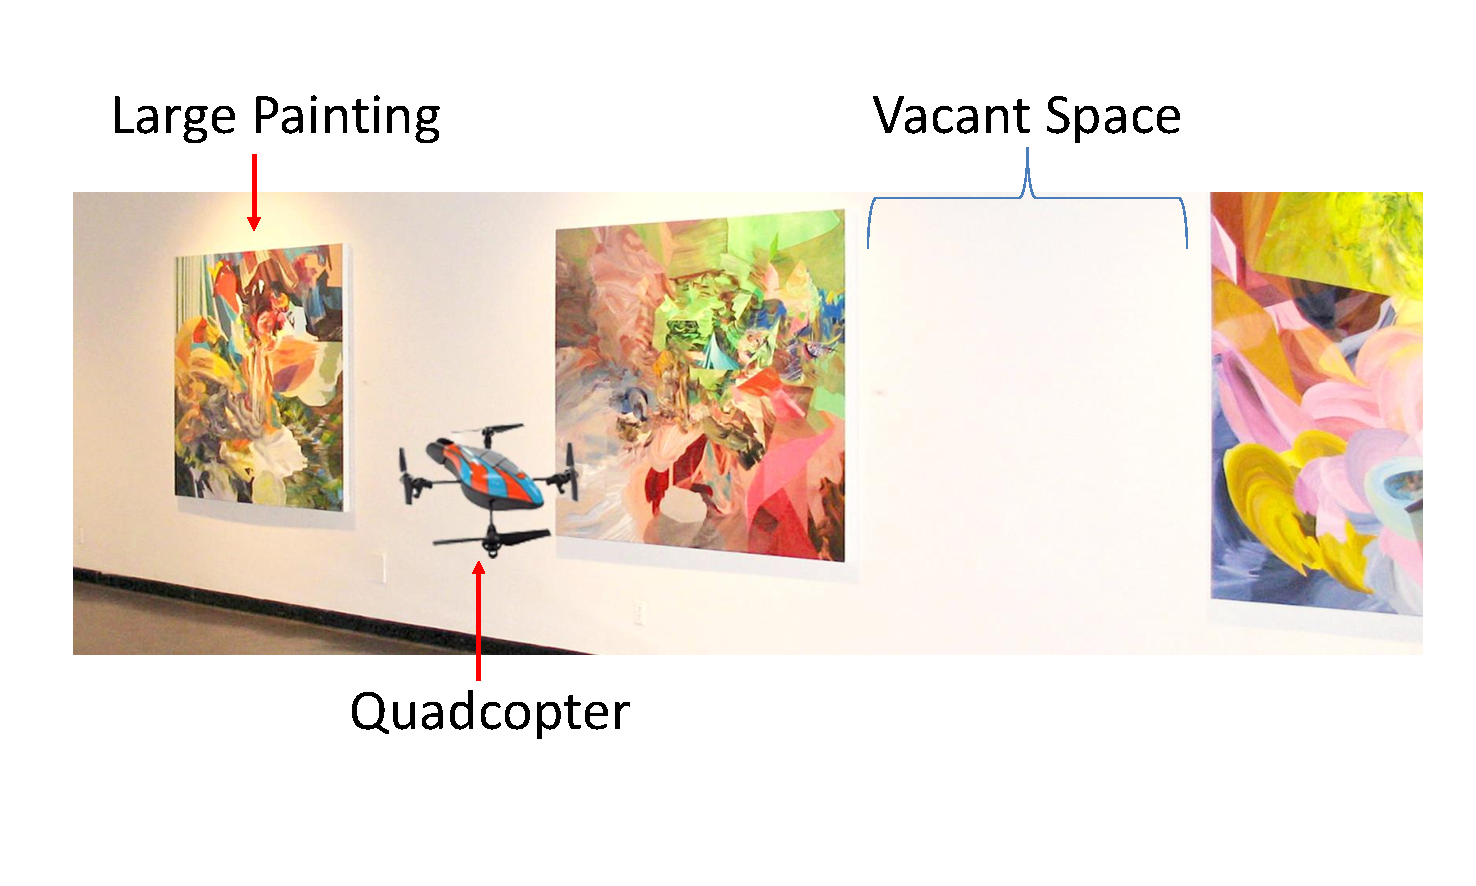
\includegraphics[width=0.49\textwidth]{mosaicing/figures/indoor}
  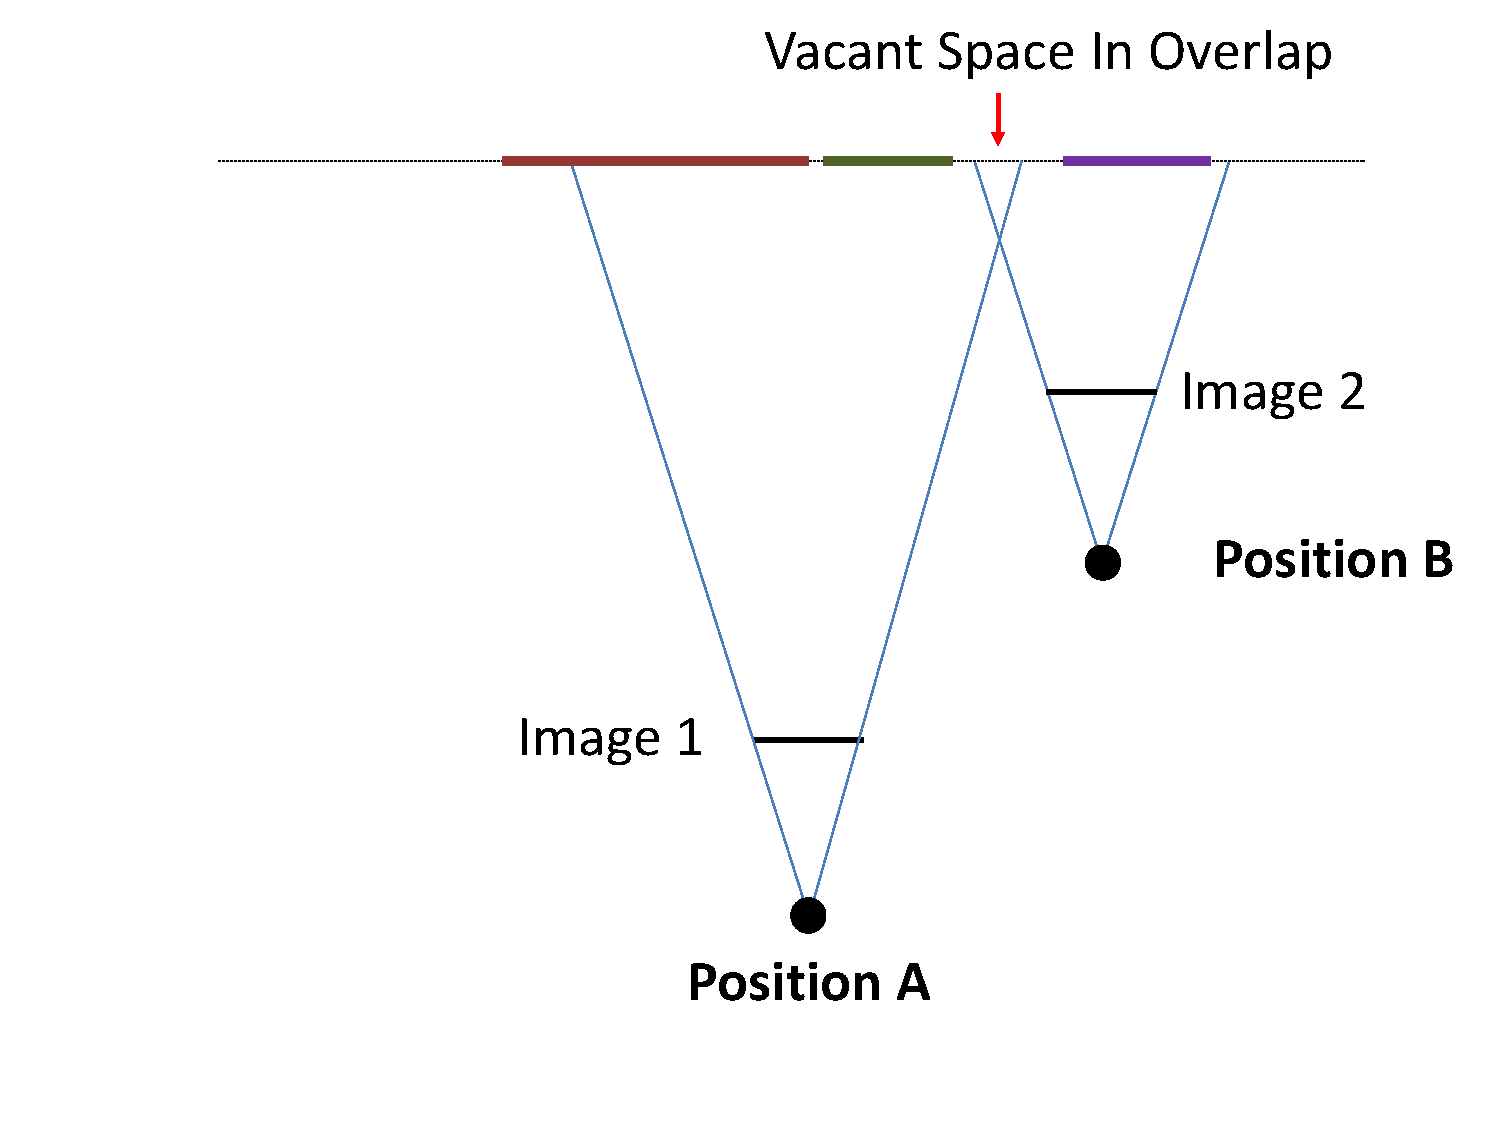
\includegraphics[width=0.49\textwidth]{mosaicing/figures/stereoOverlap}

  \caption{ \label{fig:schematic} Problem definition. (Left) Vacant spaces
    are encountered in various scenes.  When individual portions are
    captured by a quadcopter, how does one create the complete mosaic
    given that common features are either not available, or
    confusing?\\
    (Right) Simplified reduction of the problem to a geometrical structure.
  }
\end{figure}    

The method adopted is pictorially depicted in the overview shown in
Figure~\ref{fig:workflow} and is described in detail later on.  In
brief, we systematically acquire a video of the scene, reduce the large
number of images into a manageable number, and finally combine the
images acquired from different positions into a mosaic.

\begin{figure}[h!]
  \centering
  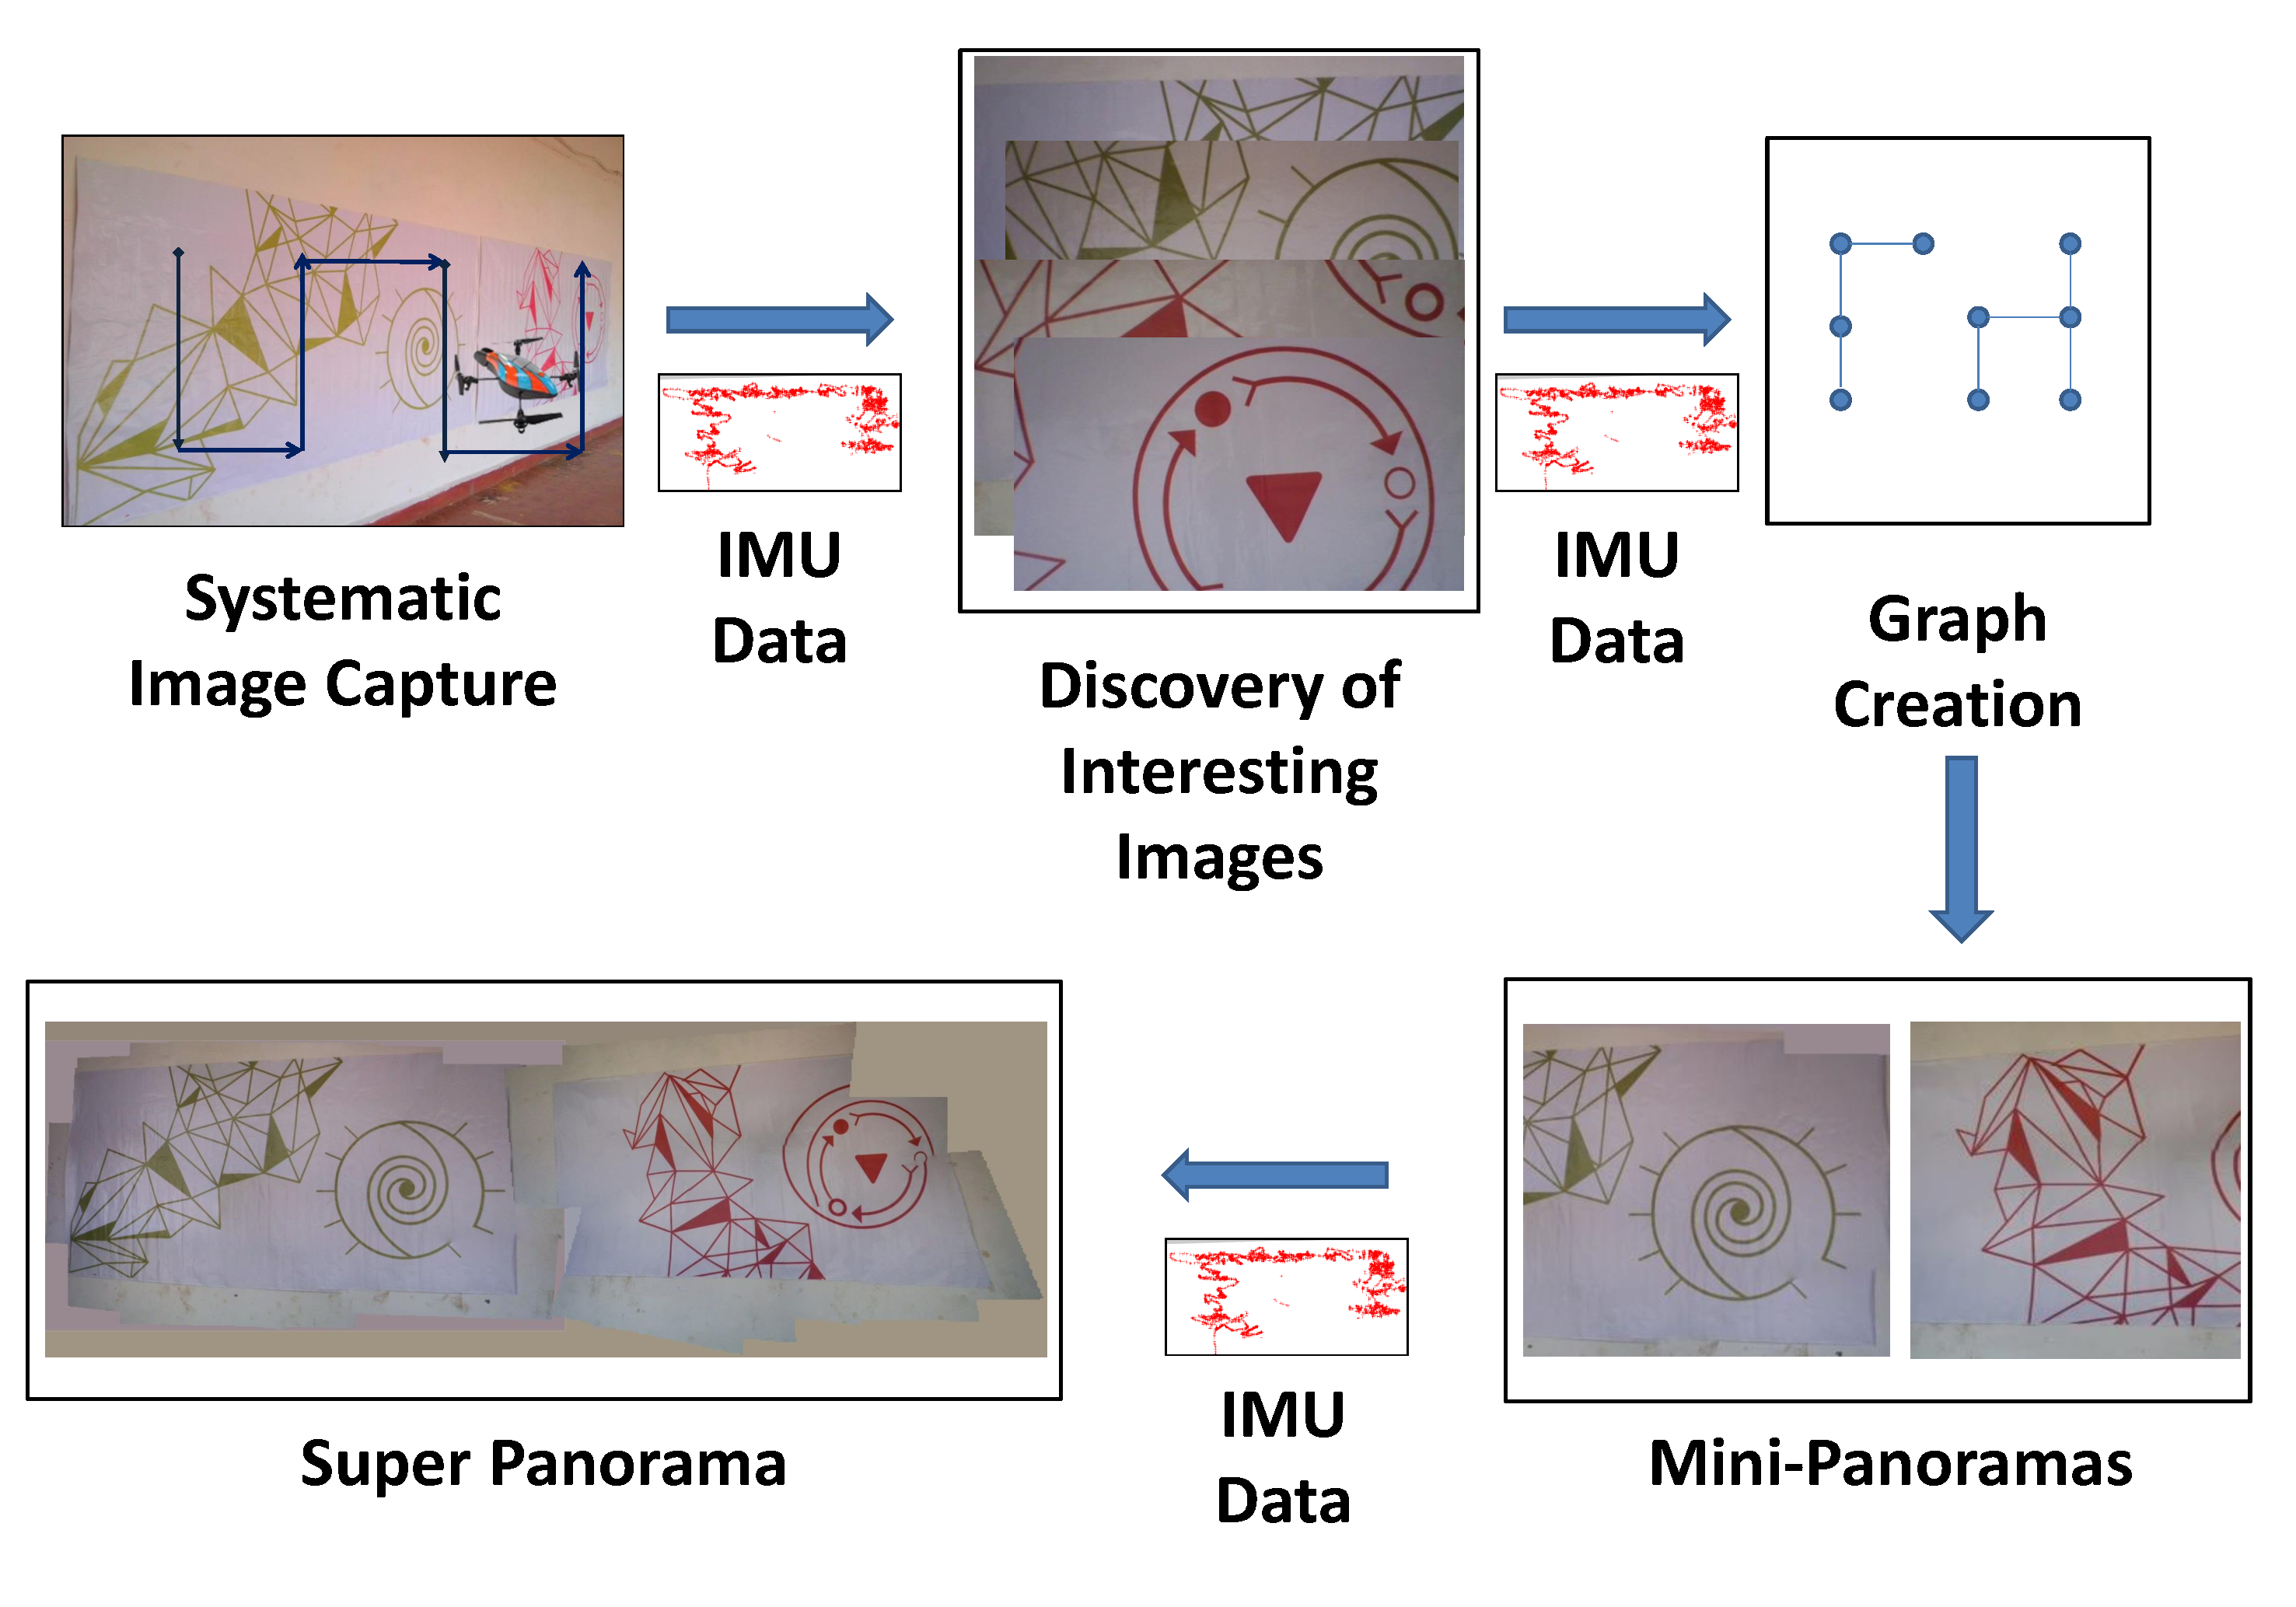
\includegraphics[width=\textwidth]{mosaicing/figures/Workflow} 
  \caption{ \label{fig:workflow} Overview: Input imagery is
    systematically acquired (top left) by a quadcopter.  In the next
    step, interesting images are found by clustering the video into
    regions based on positional data.  A graph is constructed using
    proximal images. For each connected component in a graph, standard
    stitching techniques are used to create mini-panoramas which are
    then joined together into super panorama 
    again using IMU data.}
\end{figure}    

\noindent\textbf{Video acquisition}
We first despatch the quadcopter to as close to the scene as
possible. The corners of a rectangular area of interest is provided to
the quadcopter, and it is programmed to traverse the area in a snake
like raster scan fashion.  There are various control aspects involved
in sending a quadcopter; in outdoor areas, the quadcopter is impacted
by wind and it might lose its way.  The control aspects of the
quadcopter is discussed in Section \ref{sec:furtherWork}.

The quadcopter returns with a video of the scene.  Any short video of
about a minute or more when given to a stitching program such as
Autostitch overwhelms the program, rendering it unusable. In the rest
of this section, we use Autostitch to indicate state of the art
stitching programs such as Autostitch, Photoshop, etc.

\noindent\textbf{Acquiring interesting images}
\label{sec:selection}
Our goal in this step is to reduce the amount of input data and
produce a set of interesting images.  In other words, we wish to
convert a video into an album of images.  The key difference between
our problem and standard albumization \cite{Aner, Lee} is the use of 
positional information.  A standard quadcopter has an inertial
measurement unit (IMU) that, after calibration, can give accurate
information of positions.

Using this it is possible to cluster the images, and sort the images
into an $m\times n$ grid.  (Occasionally we have encountered outlier
situations and thus erroneous positional information.  Thus we believe
standard vision-based clustering method can be used to either drop
frames, or to correctly include frames based on image content.)  The
number of cluster centers is automatically determined using the
agglomerative bottom up hierarchical clustering method \cite{Lior}, with the
additional requirement that the whole scene (represented by the
positional data) is covered.  

{\bf Clustering Details} We assume that each IMU data position
corresponds to an image of definite fixed dimensions.  Consider each
position of the IMU data to be a leaf node. Two nodes are greedily
combined based on the closest Euclidean distance, and replaced with an
internal node.  The position of the internal node is set to be the
centroid of the two nodes, and each internal node now corresponds to a
virtual image taken by a virtual quadcopter.  The algorithm
recursively merges all the nodes till we end up with a root.  In the
next phase, we proceed top-down and level by a level to find the
cluster centers.  A set of nodes is considered for being the output as
cluster centers if the union of these nodes completely cover the
scene. From the bottom-up construction, it is clear that the root will
represent a single position, and thus a single image and most likely
will not cover the scene.  At the other extreme, the set of all leaf
nodes \emph{will} cover the scene.  The top-down algorithm proceeds
from root and finds the minimal set of nodes which cover the scene.
Once cluster centers are found, we pick the leaf node which is closest
to the cluster center to find a real image.
This process is pictorially described in
Figure~\ref{fig:selection}.


\begin{figure}[h!]
  \centering
  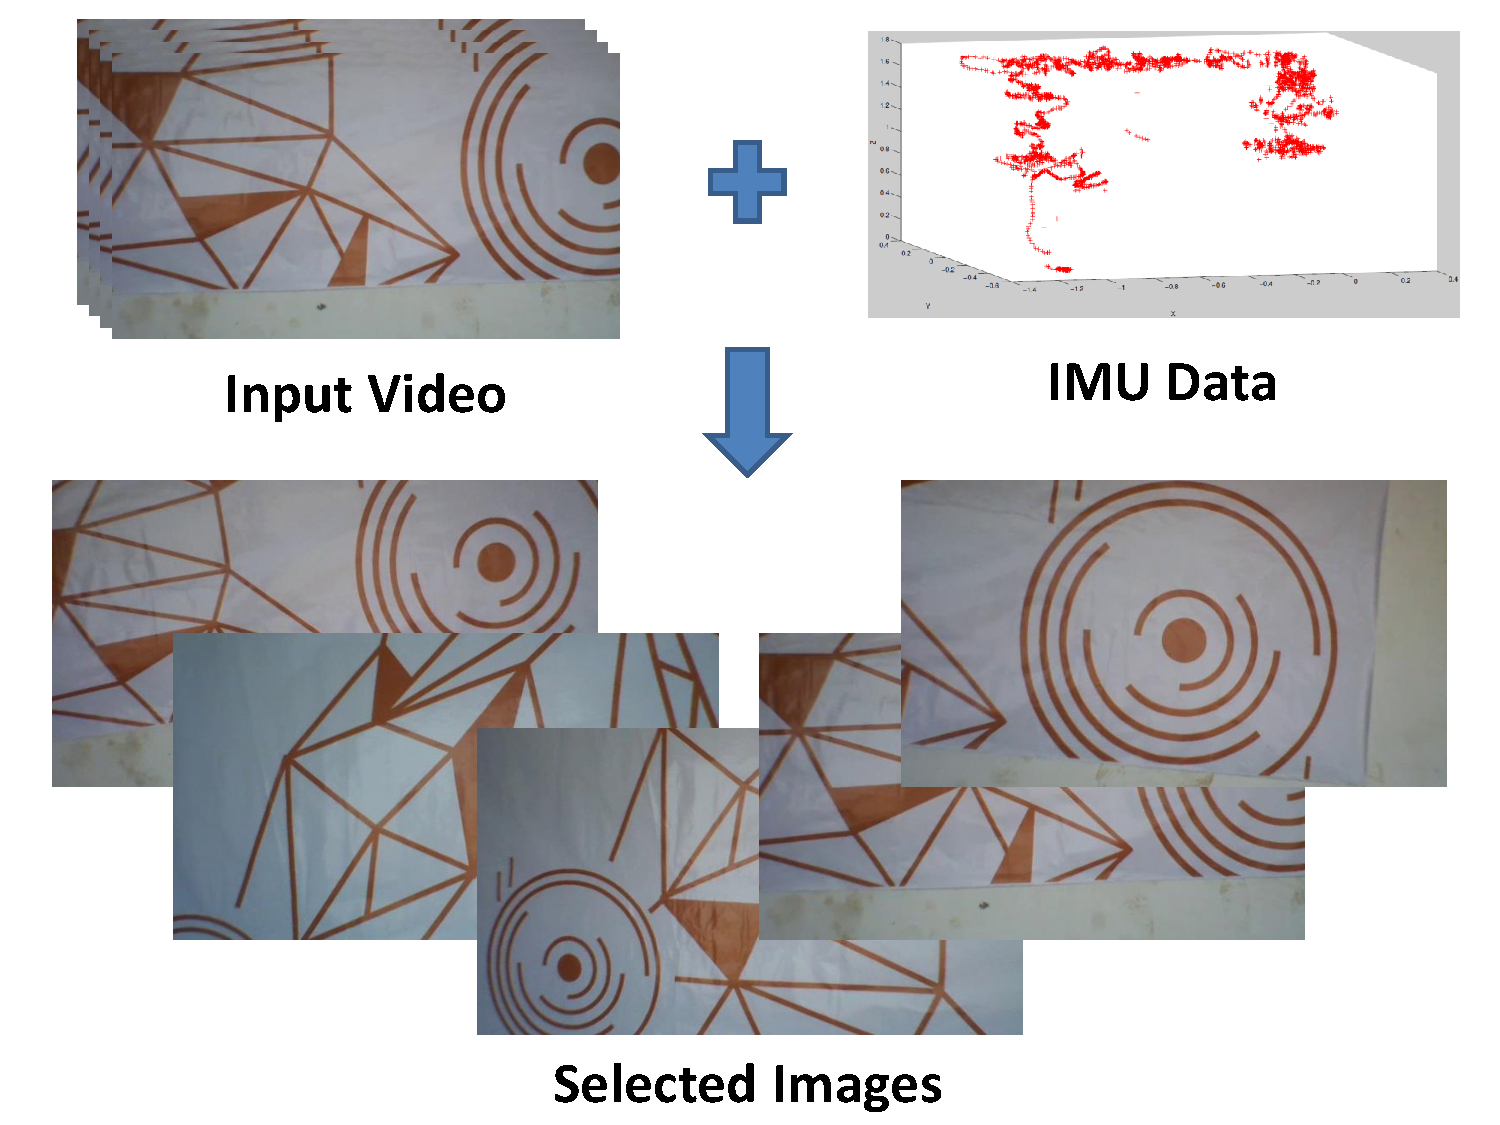
\includegraphics[width=\textwidth]{mosaicing/figures/selection} 
  \caption{ \label{fig:selection} Using IMU data, an image stream is
    transformed into a set of interesting images for purpose of
    panorama creation. }
\end{figure}    

In practice, the number of cluster centers for the scenes we have
covered is now within the capacity of Autostitch.  As mentioned in the
introduction, as long as there are sufficiently varying and
``matchable'' features, Autostitch is able to perform a reasonable
result.  However, if there are very few features in overlapping region
of two images, then the output is not acceptable. This situation will
arise when there is vacant space between two pictures.

{\bf Time complexity} Autostitch has not been designed
to use positional information. As a result if there are $N$ input
images, the program has to consider possible matches in approximately
$O(N^2)$ set of areas.  Our program is able to mosaic in an $O(N)$
fashion.

% MSB - There are no details to the clustering, or the "postulating" of edges.
{\bf Spanning Trees}
Specifically, we assume at this point that the interesting photos are
available in the form of a $m \times n$ grid. First, we find SURF
\cite{Bay} features for each image in a grid. Next, we use Best of
Nearest Neighbor matcher (from the OpenCV library) with Random Sample
Consensus (RANSAC) \cite{Fischler1981} to find geometrically
consistent matches between neighborhood images inside grid.  We
create a graph with images being nodes, and add an edge between two
nodes if there are sufficient matches. We have to recall at this point
that if there are ``vacant spaces'' there will not be enough features
for successful matches; the graph will end up with multiple
(disconnected) components.  We next compute multiple spanning trees
for the various components. Given a spanning tree, the center of the
spanning tree is a node from which the distance to all other nodes is
minimal \cite{Kocay}. Next we calculate the homography of each image with respect
to spanning tree center.  Finally, for each spanning tree, we stitch
all pictures using the computed homographies by warping all images
with reference to the image at spanning tree center. The spanning tree is
an $O(N)$ structure. The process is described in
Figure~\ref{fig:graph}.

\begin{figure}[h!]
  \centering
  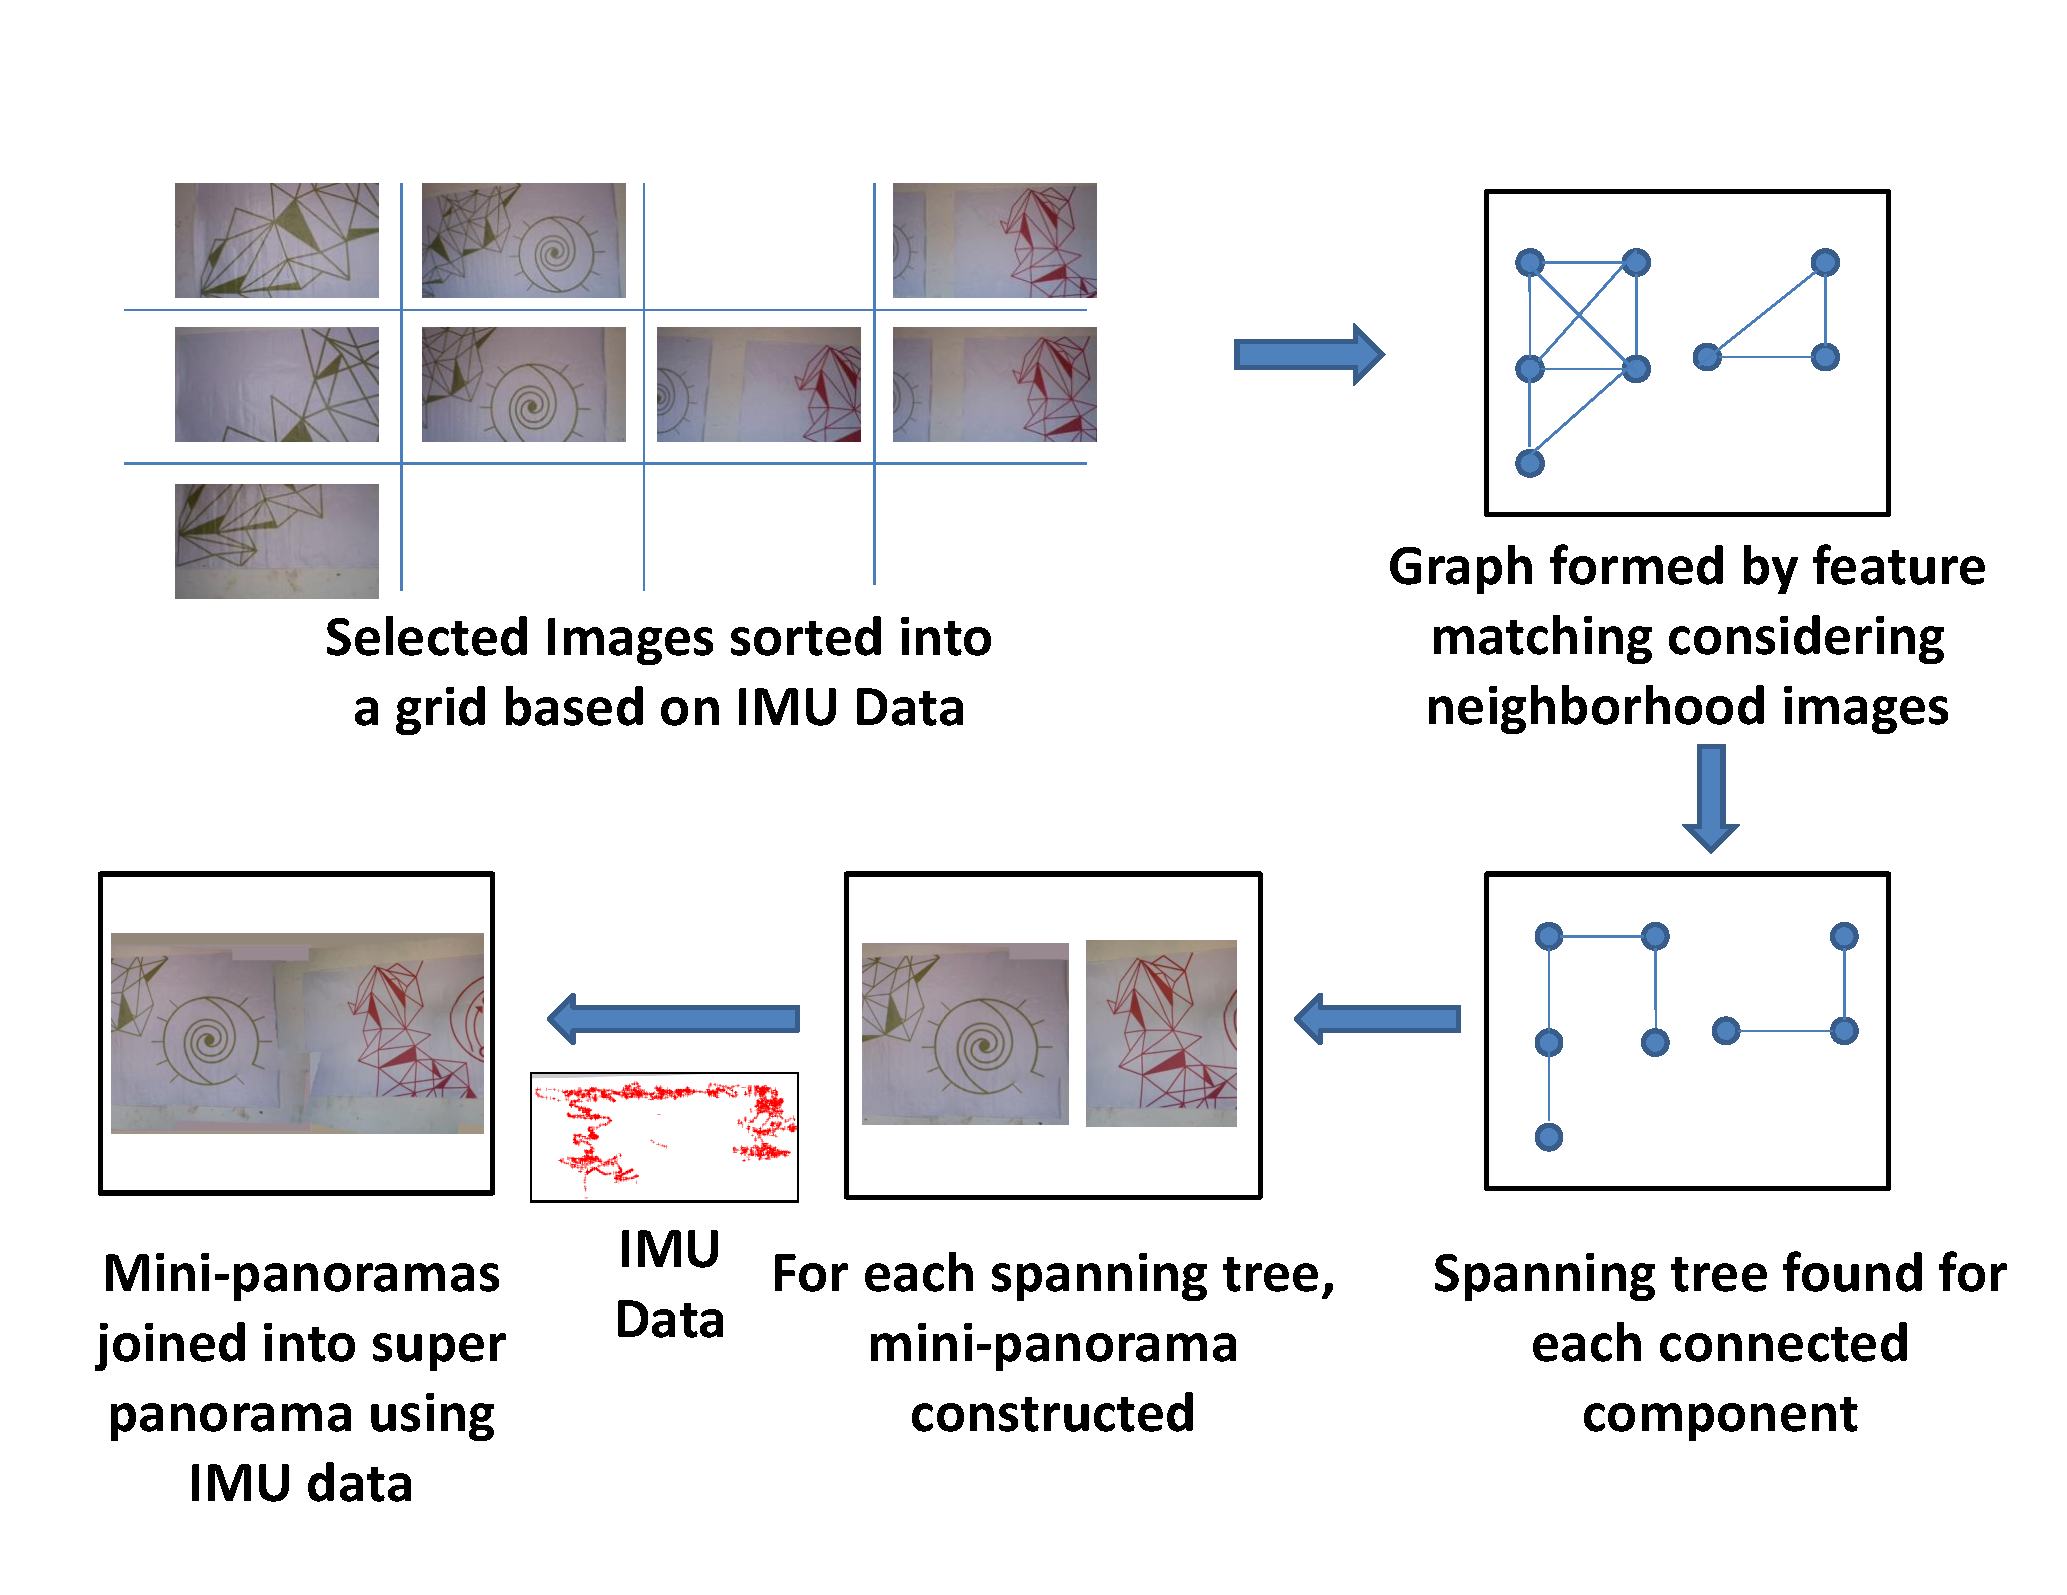
\includegraphics[width=\textwidth]{mosaicing/figures/graphCreation} 
  \caption{ \label{fig:graph} Interesting images acquired are
    segmented and individual (mini-panoramas) are constructed. These
    are then later combined into the desired super-panoramas using IMU data.}
\end{figure}    

\noindent\textbf{Super-panoramas}
  
In this section, we consider the situation when programs like
Autostitch fail.  We assume that the output of the previous step has
resulted in multiple spanning trees where each spanning tree center
corresponds to a specific depth. This is the depth of the center of
the spanning tree, since we have stitched all images by taking the
spanning tree center as a reference.  Individual panoramas for each
spanning tree termed mini-panoramas have been created. A
super-panorama must be created from mini-panoramas; these usually
correspond to different depths for at least two reasons.

First, it is invariably difficult, if not impossible, to control a
quadcopter to be at the exact depth even in indoor scenes.  The
aerodynamics and the thrust produced tends to make the quadcopter
drift.  Second, it might also be necessary to let the quadcopter probe
and come closer to the scene so as to get a ``good picture''.

A super-panorama is done using a two step process. Assume two trees in
the forest corresponding to area A and area B of the scene (see
Figure~\ref{fig:stereo}). 
\begin{figure}[h!]
  \centering
  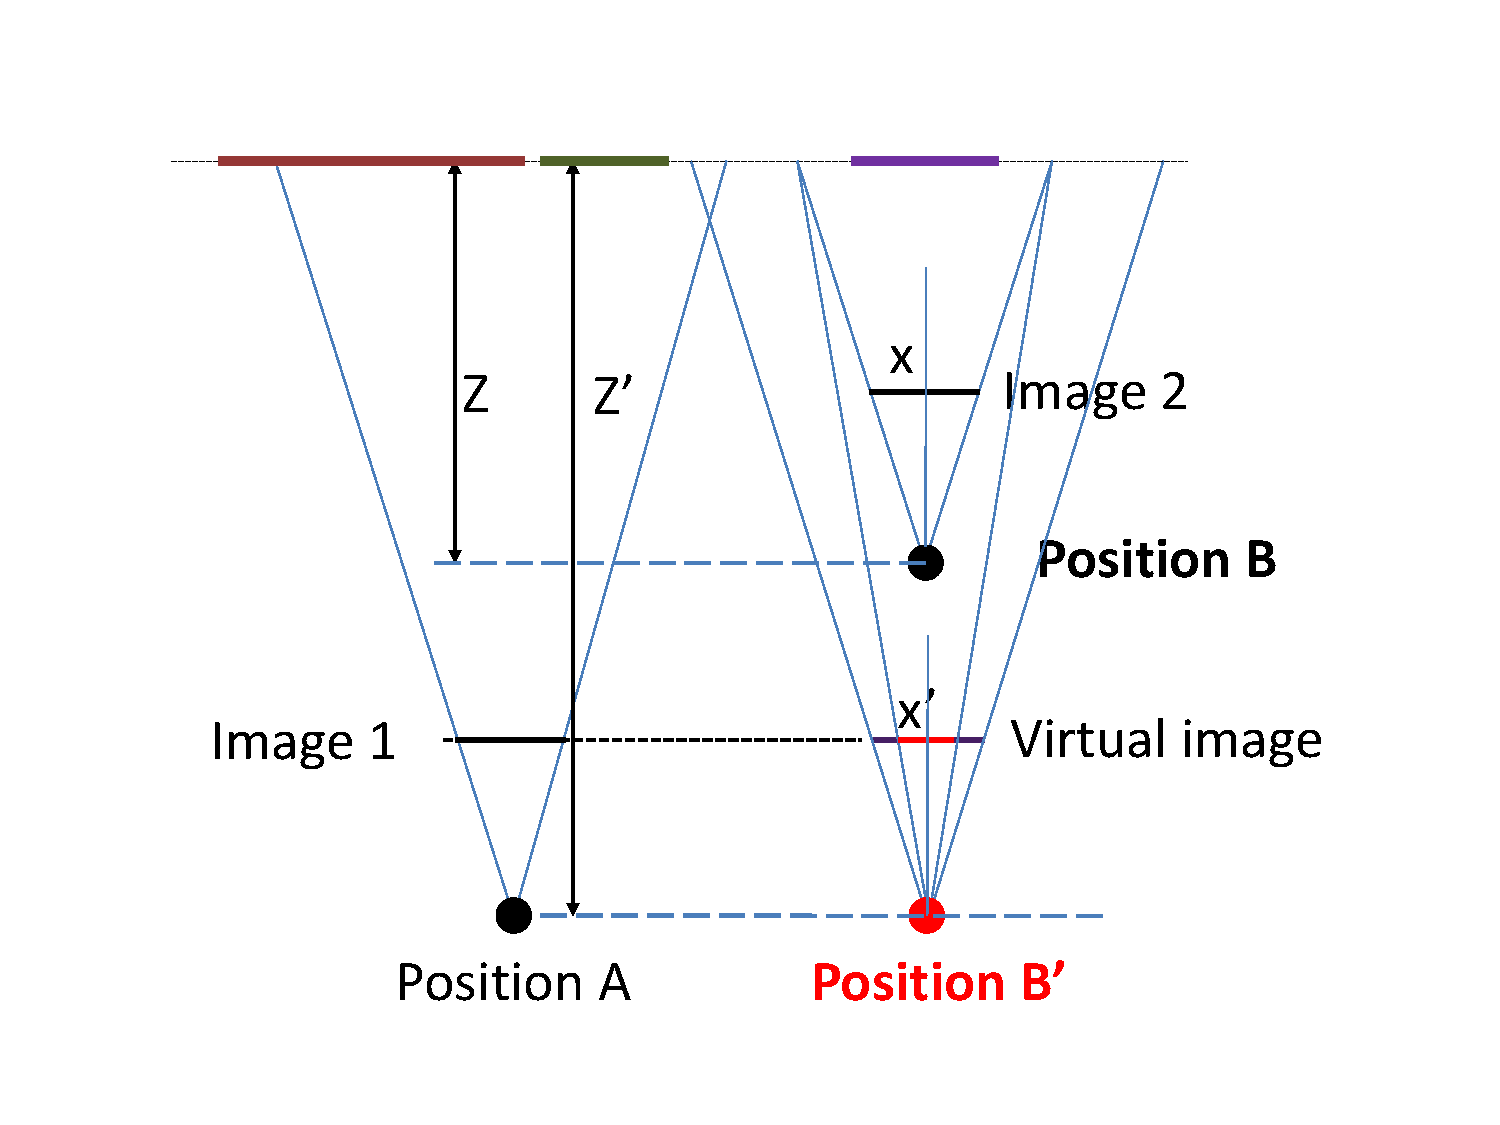
\includegraphics[width=0.45\textwidth]{mosaicing/figures/move} 
  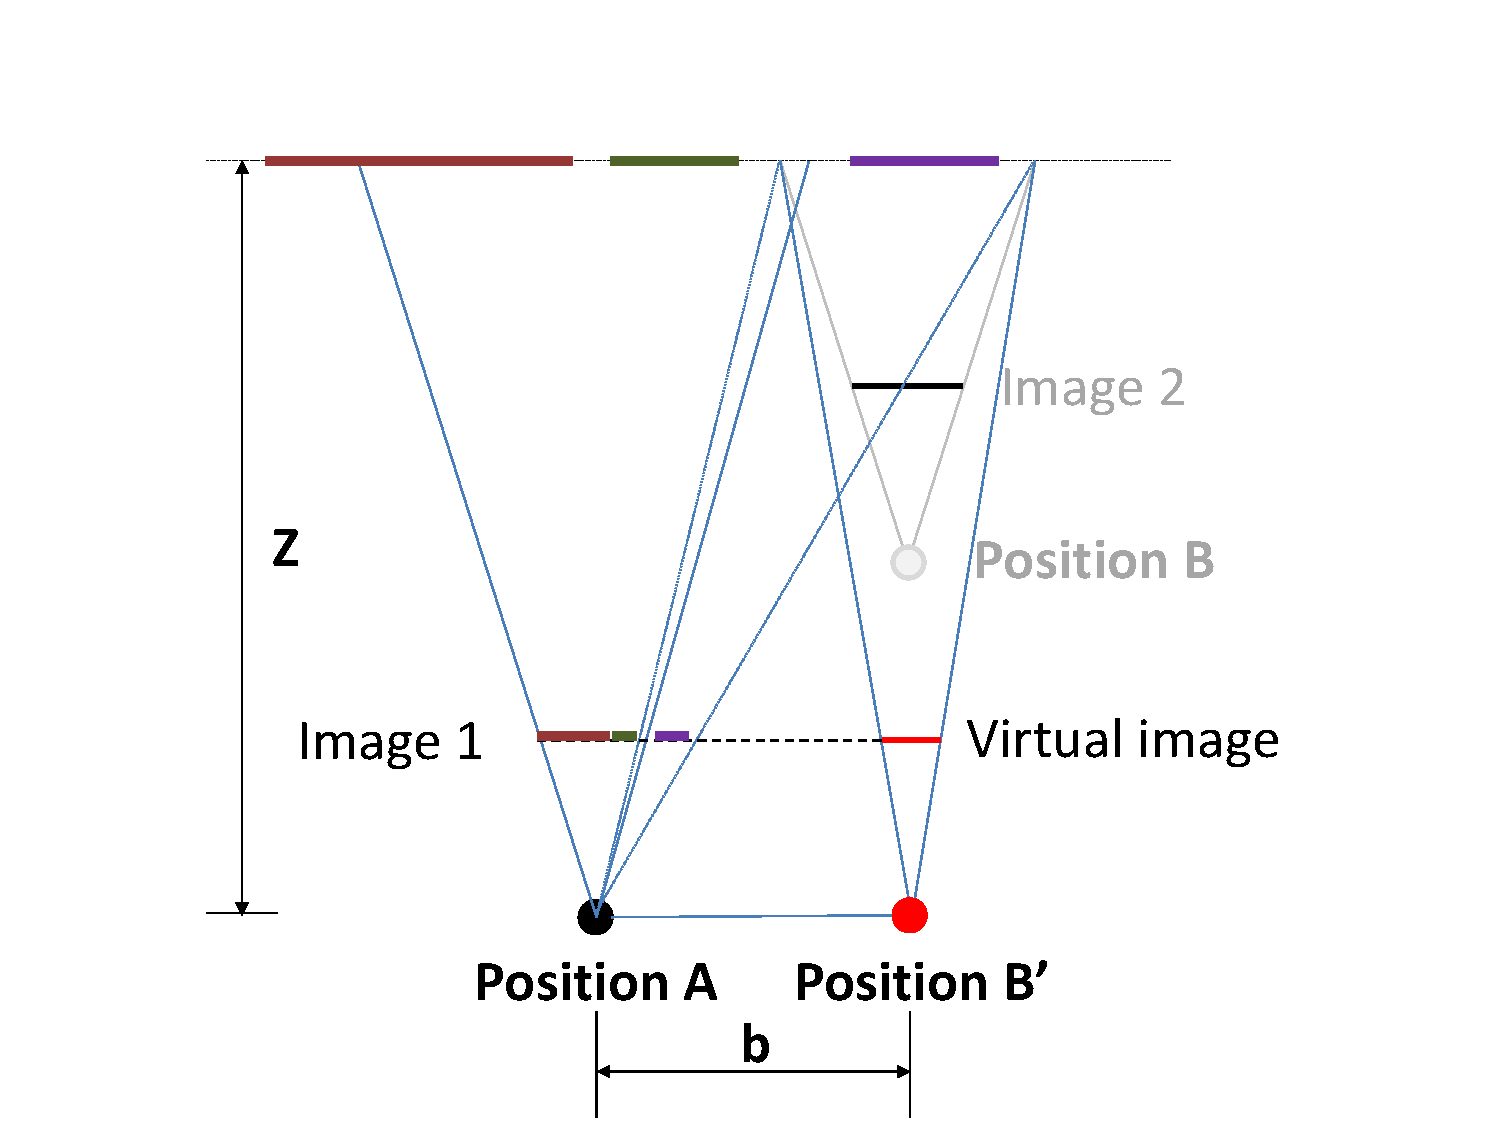
\includegraphics[width=0.45\textwidth]{mosaicing/figures/stereo} 
  \caption{ \label{fig:stereo} (Left) The virtual picture as seen from position
  B' is computed using Equation~\ref{eq:moveRelation} from the real picture
    taken from B.  (Right) Using the disparity, and the baseline width,
  it is possible to depict the composite scene obtained from both A
  and B' (from the view point of A).}
\end{figure}    
Assume that a mini-panorama is created from these two areas, and the
depth of the planar surface from the camera is more for A, than for
B. We then take the mini-panorama image captured at B, and `move' it to
a new location B’ whose depth (from the imaged surface) is the same as
that of A. The resulting image  will be smaller; the images are
related by the equation
\begin{equation}
  \label{eq:moveRelation}
  {\bf \frac{x'}{x} = \frac{Z}{Z'}}
\end{equation}
where {\bf x} (respectively {\bf x'}) represents a pixel location of
the image in B (respectively, B') and 
{\bf Z} (respectively {\bf Z'}) represents the depth of the images
surface from B (respectively, B').

We can now treat the resulting images from A (unchanged) and B’
(computed from Equation~\ref{eq:moveRelation}) forming a stereo pair.
Using the stereo disparity formula we can ``place,'' from the view
point of A, the image captured from B, thereby creating a
super-panorama.

\subsection{Experiments and Results}
\label{sec:results}

All our experiments have been completed with the inexpensive consumer
quadcopter called a Parrot's AR Drone 2.0. We have used the ROS based
ARDrone Autonomy Driver to communicate with the drone. For the purpose
of showing the efficacy of our method, we also took a picture of the
scene from a distance with a 5 mega-pixel camera to better understand
the scene.

We have implemented our algorithm in C++ using the OpenCV library
(OpenCV 2.4.9). Experiments were performed on a PC with Intel Core i7
processor(@3.4GHz) and 8GB RAM.

\noindent\textbf{Selecting Images}

In our first experiment, we wanted to ensure that the selection of
images done was comprehensive and useful.  We sent the drone to image 
an outdoor scene with no vacant space. This experiment was conducted
in an outdoor environment. We note here that there were approximately
3000 images in the raw video.  Autostitch was unable to cope  when fed
with this large number of frames.

One way to produce some sort of mosaic was to simply reduce the amount
of data given to Autostitch.  Figure~\ref{fig:sac3}(a) shows uniformly
(time) sampled images from the video.  When these sampled images are
given to Autostitch or to Adobe Photoshop, we find
(Figure~\ref{fig:sac3}(b)) that these programs are able to produce
some output, but the results are not satisfactory.

Instead of feeding time-sampled images, we ran our saliency selection
algorithm (as explained in Section~\ref{sec:selection}) on the video
which resulted in $N = 5$ images.  Though the number of input images
in the video is large, the total distance covered by the quadcopter in
this duration (of around 90 seconds) is small; thus the
number of distinct images returned by the algorithm shows a dramatic
reduction. Figure~\ref{fig:sac3}(c) shows examples of selected images.
Many of the images are similar to the time sampled version; however,
the occasional differences are enough to make Autostitch work. The
results are shown in Figure~\ref{fig:sac3}(d).

\begin{figure*}[h!]
\centering
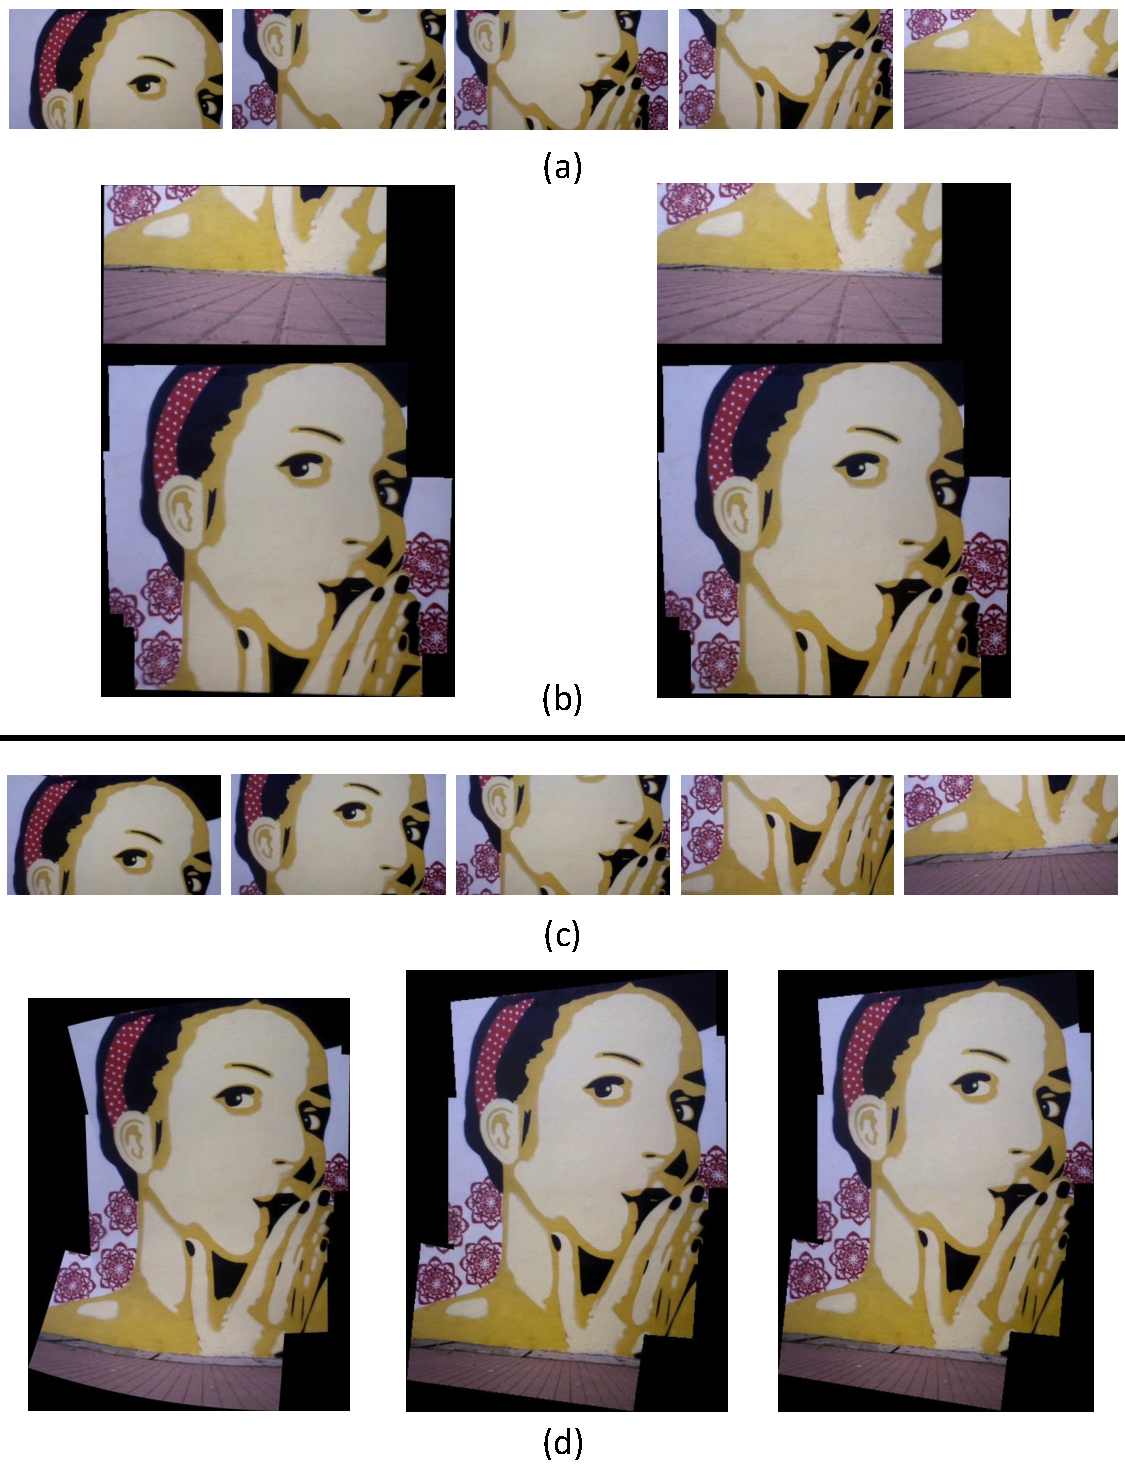
\includegraphics[width=0.87\linewidth]{mosaicing/results/ValidationResult}
\caption{ (a) Uniformly sampled images from an outdoor video
  expedition.  (b) Output of the state of the art photo stitchers
  (left:Autostitch, right:Adobe Photoshop CS6) on uniformly time
  sampled images.  As time sampled images do not guarantee coverage of
  the scene, the panorama is broken. The top portions do not belong at
  the right place (see (d)) (c) Salient image selection from the set of
  approximately 3000 images using positional information. (d) When
  salient images are given to Autostich (left) and Photoshop (middle),
  we can create a panoramic mosaic (since there are no vacant
  spaces). We also show the result from our stitching algorithm
  (bottom right).}
\label{fig:sac3}
\end{figure*}

We tested our salient image selection algorithm on another
input stream which had about 9000 images. The selection algorithm of Section
\ref{sec:selection} pruned the video into $N=15$ images. The scene as captured
by a typical camera can  be seen in Figure~\ref{fig:validResults}(a). A sample
of the selected images are seen in Figure~\ref{fig:validResults}(b).
Figure~\ref{fig:validResults}(c,d,e) shows the comparison of outputs of the state
of the art stitching methods with the output of our algorithm. The input scene
is such that there are no vacant spaces; our stitching algorithm's output is
similar to that of Autostitch \cite{autostitch} as well as Photoshop
\cite{photoshop}. Results on this dataset again demonstrates that programs like
Autostitch, Photoshop can correctly stitch images selected by our algorithm
(when there are no vacant spaces).

\begin{figure}[h!]
\centering
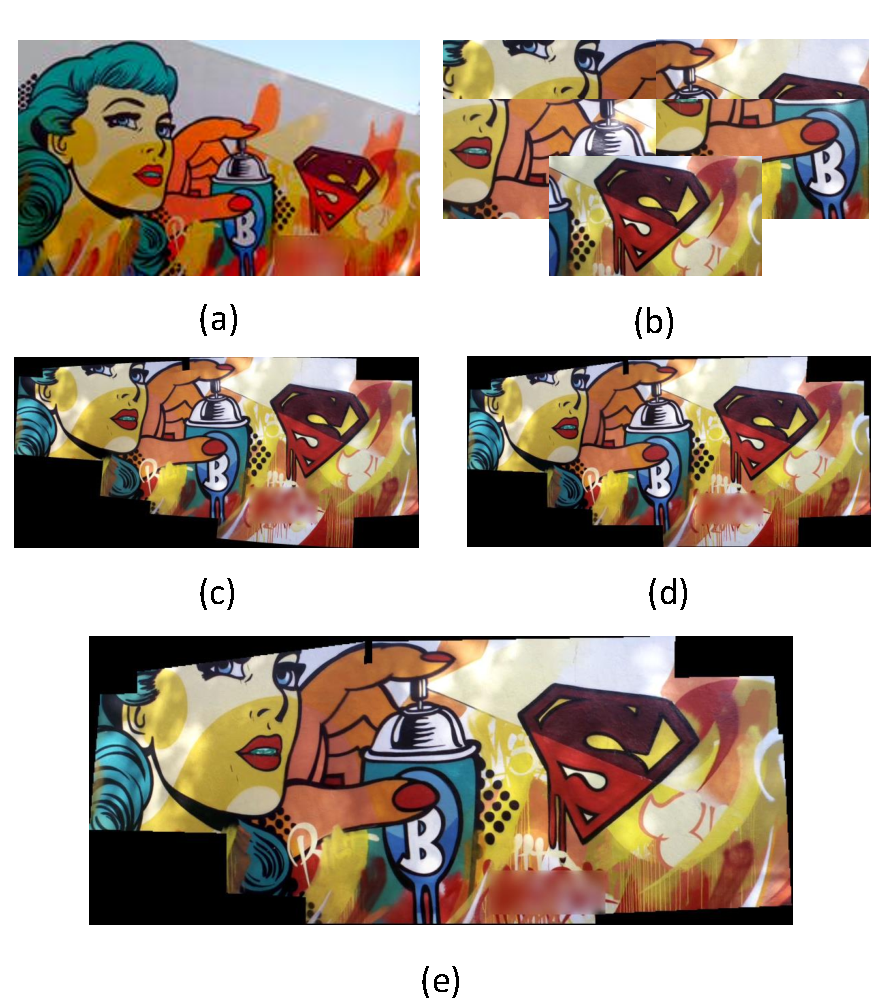
\includegraphics[width=0.87\linewidth]{mosaicing/results/sac1}
\caption{ (a) An outdoor scene captured by a standard camera.  (b) Salient image selection from the set of
  approximately 9000 images using positional information. (c) Output of
  Autostitch \cite{autostitch} on the images selected by our algorithm. (d) Output of Adobe Photoshop CS6
  \cite{photoshop} on the selected images. (e) Output of our method.}
\label{fig:validResults}
\end{figure}

In summary, these experiments provides evidence to show that (a) our
saliency selection algorithm is reasonable and (b) our stitching
results are comparable to that of Autostitch for the kind of scenes
considered.

\noindent\textbf{Indoor Imagery with Vacant Spaces}

Our next selection of experiments were conducted in an indoor
environment.  The input stream had about 4300 images. The selection algorithm
(Section~\ref{sec:selection}) pruned the video into $N=4$ images.
A sample of the selected images are seen in Figure~\ref{fig:teaser}.

\begin{figure}[t!]
  \centering
  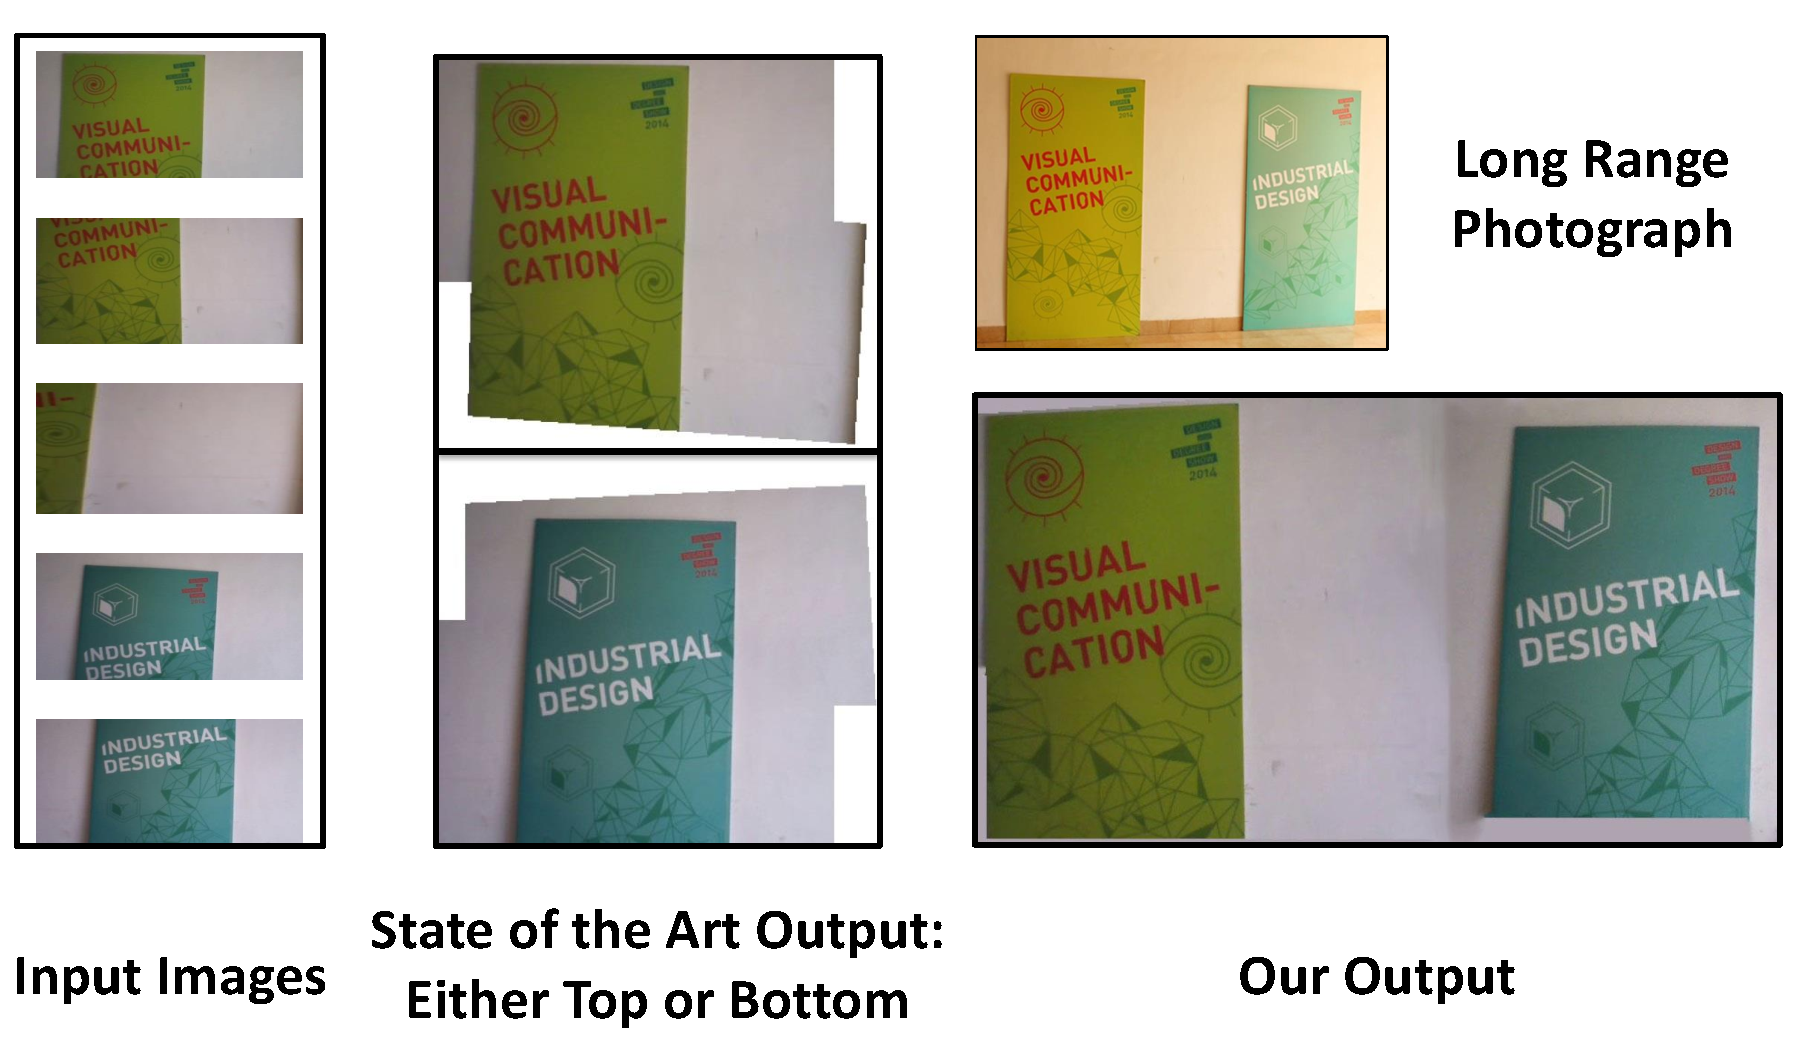
\includegraphics[width=\textwidth]{mosaicing/figures/teaser.pdf}
  \caption{ \label{fig:teaser} The long range photograph of a scene when probed
    by a quadcopter results in the input images shown on the left.  The
    state of the art methods (middle column) are unable to make a mosaic because the
    vacant space (third picture on the left) does not seem to have any
    matchable features with subsequent input images.}
\end{figure}

There were two disconnected components in the resulting graph.
Autostitch was unable to produce any reasonable output as seen in
Figure~\ref{fig:teaser}.  The scene, captured from a distance is also
shown.  One can see a better orthographic view of the posters.
\vspace{0.5cm}

\noindent\textbf{Outdoor Imagery with Vacant Spaces}
Our next set of experiments were conducted in an outdoor
environment. The input stream had about 12000 images. The selection
algorithm pruned the video into $N=30$ images. A sample of the
selected images are seen in Figure~\ref{fig:results}.  The scene as
captured by a smartphone can also be seen, as well as the comparison
of outputs of state of the art stitchers with output of our
algorithm. Figure~\ref{fig:results} shows the comparison of outputs of
state of the art stitchers with the output of our algorithm.

\begin{figure}[h!]
\centering
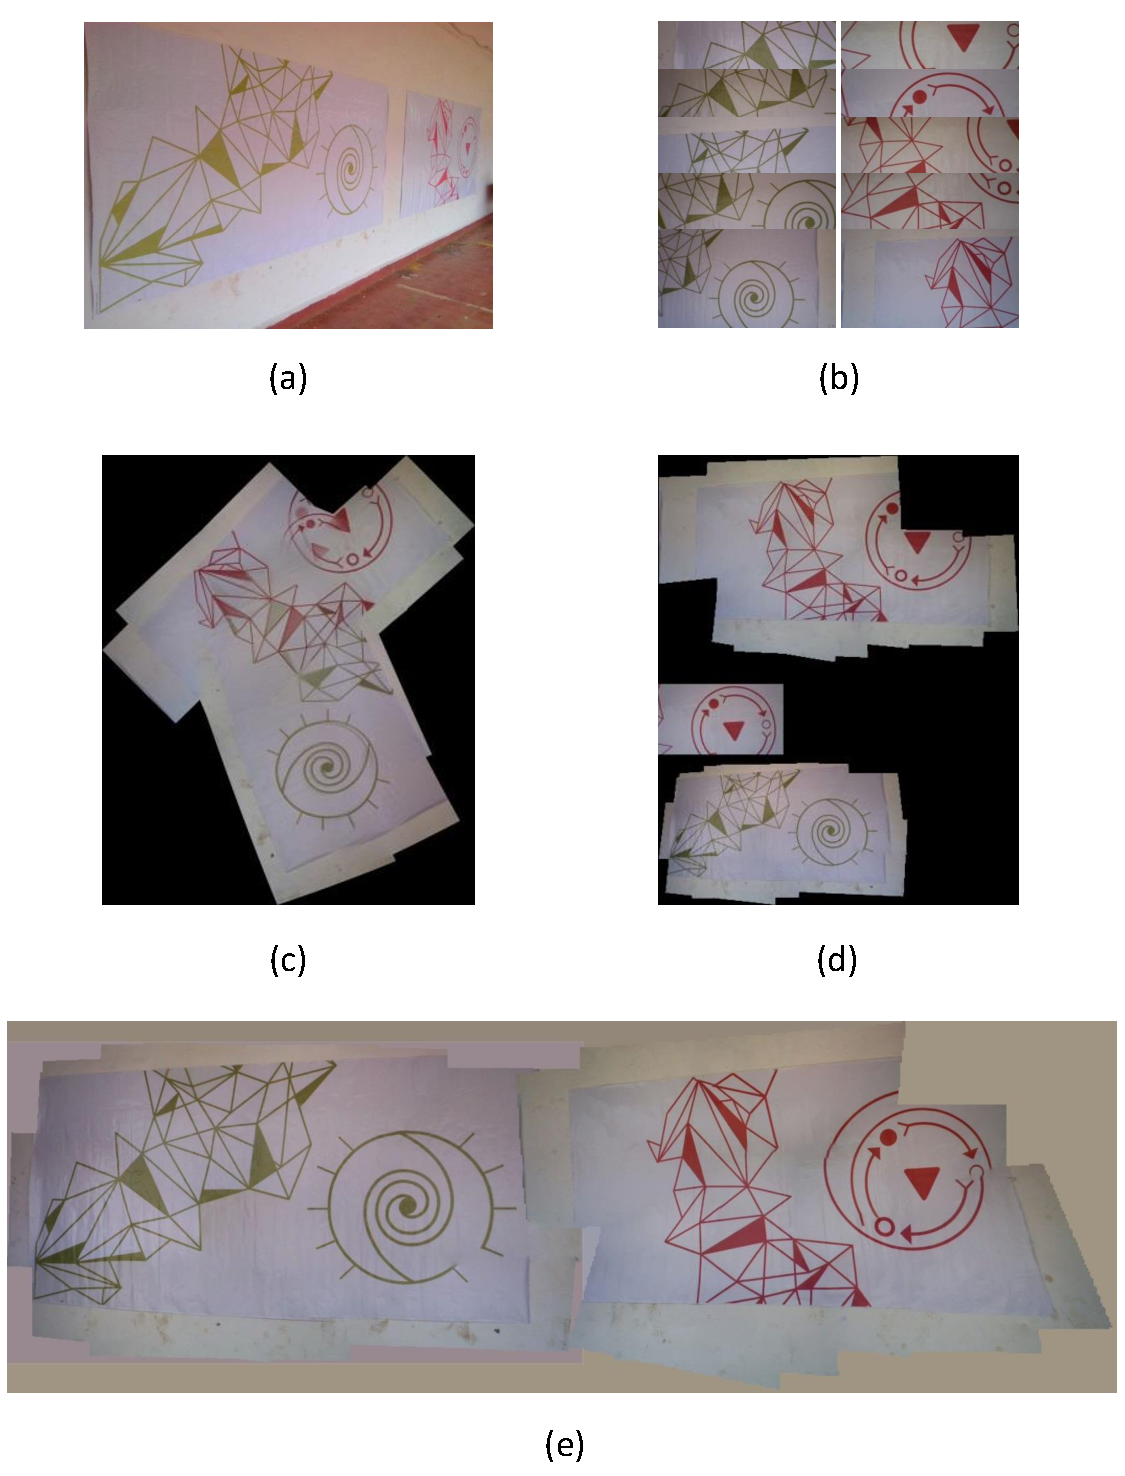
\includegraphics[width=0.86\linewidth]{mosaicing/results/results}
\caption{(a) An outdoor scene captured by a standard camera in an
  exhibition. The approach to the area is normally cordoned off and one
  needs permission to get a quadcopter to take the picture.  Notice a
  significant gap between the two posters.  (b) Pruned images from the
  quadcopter video using our saliency algorithm. (c) Output of
  Autostitch on the selected images. The mosaic is not reasonable
  presumably because of the confusion in features. (d) Output of Adobe
  Photoshop CS6 on the selected images. The vacant space posed a
  problem to the feature matching algorithm, so instead of a mosaic,
  individual pieces were output as mini-panoramas (e) Our output on
  the selected images. We are able to join two posters (separated by
  vacant space) using IMU data.}
\label{fig:results}
\end{figure}

Next input stream had about 9100 images. The selection algorithm pruned the
video into $N=28$ images. The scene as captured by a smartphone can also be seen in
Figure~\ref{fig:results1}(a). A sample of the selected images are seen in
Figure~\ref{fig:results1}(b). Figure~\ref{fig:results1}(c,d,e) shows the
comparison of outputs of state of the art stitchers with the output of our
algorithm. As there are vacant spaces, Autostitch~\cite{autostitch} as well as
Photoshop~\cite{photoshop} are unable to stitch images accurately. In contrast,
since we use positional data, our output is an acceptable mosaic, and shows an
orthographic view.

\begin{figure}[h!]
\centering
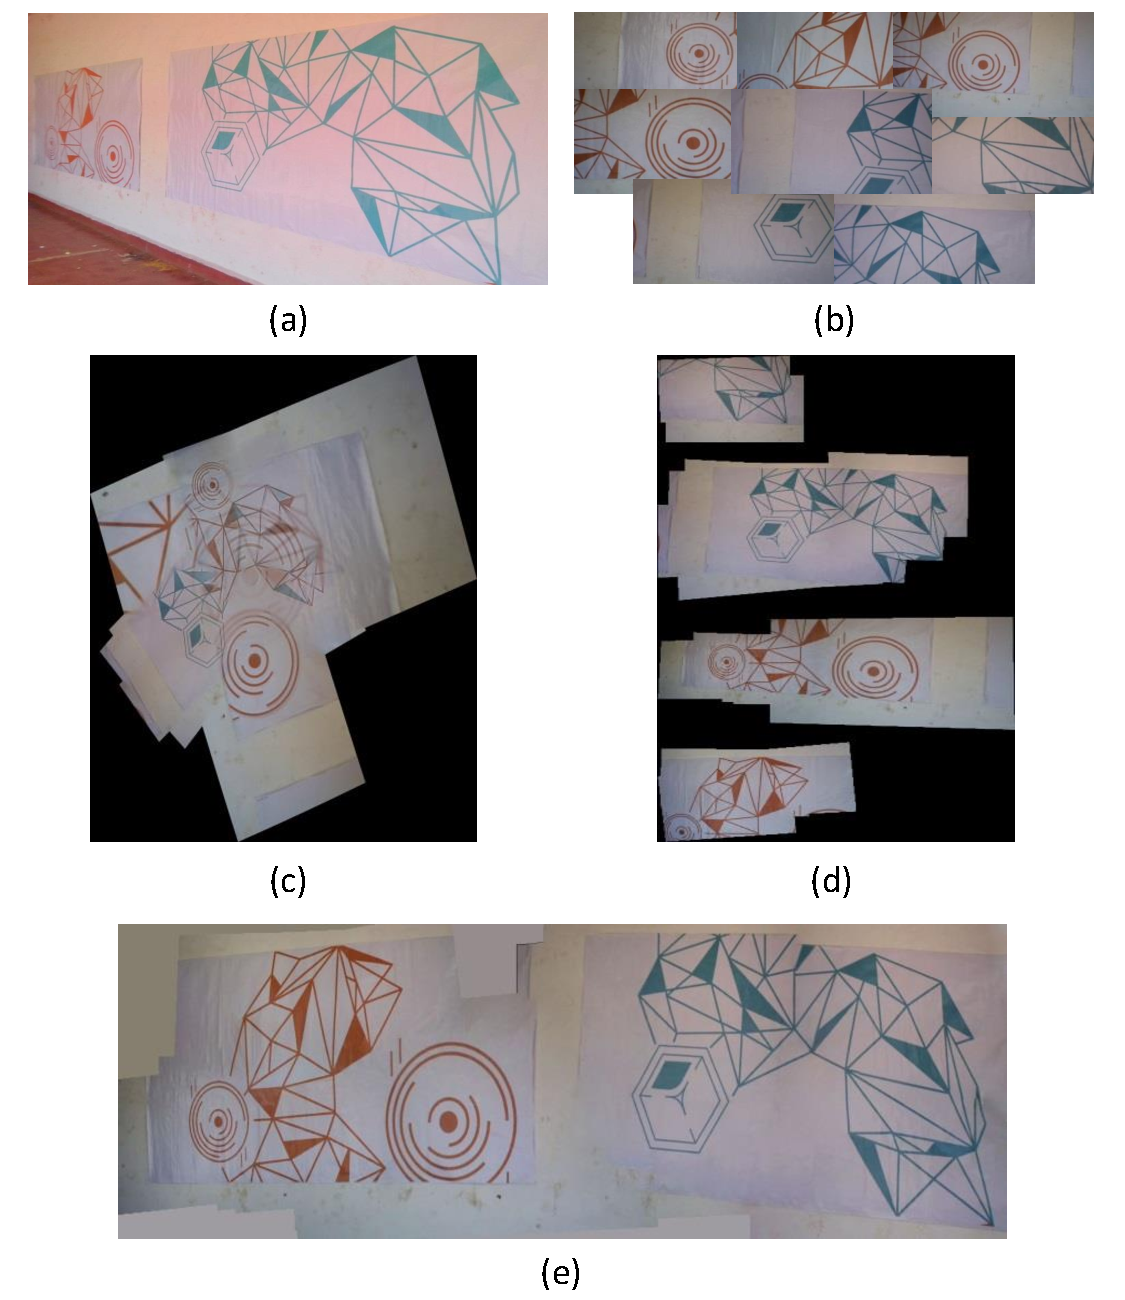
\includegraphics[width=0.85\linewidth]{mosaicing/results/orange_blue.pdf}
\caption{(a) An outdoor scene captured by a standard camera in an
  exhibition. The approach to the area is normally cordoned off and one
  needs permission to get a quadcopter to take the picture.  Notice a
  significant gap between the two posters.  (b) Pruned images from the
  quadcopter video using our saliency algorithm. (c) Output of
  Autostitch~\cite{autostitch} on the selected images. The mosaic is not
  reasonable presumably because of the confusion in features. (d) Output of Adobe
  Photoshop CS6~\cite{photoshop} on the selected images. The vacant space posed
  a problem to the feature matching algorithm, so instead of a mosaic,
  individual pieces were output as mini-panoramas (e) Our output on
  the selected images. We are able to join two posters (separated by
  vacant space) using IMU data.}
\label{fig:results1}
\end{figure}

The input stream had about 8500 images. The selection algorithm pruned the video
into $N=17$ images.The scene as captured by a smartphone can also be seen in
Figure~\ref{fig:results2}(a). A sample of the selected images are seen in
Figure~\ref{fig:results2}(b). Figure~\ref{fig:results2}(c,d,e) shows the
comparison of outputs of state of the art stitchers with the output of our
algorithm. As there are vacant spaces, Autostitch~\cite{autostitch} as well as
Photoshop~\cite{photoshop} are not able to stitch images accurately. In
contrast, since we use positional data, our output is an acceptable mosaic.

\begin{figure}[h!]
\centering
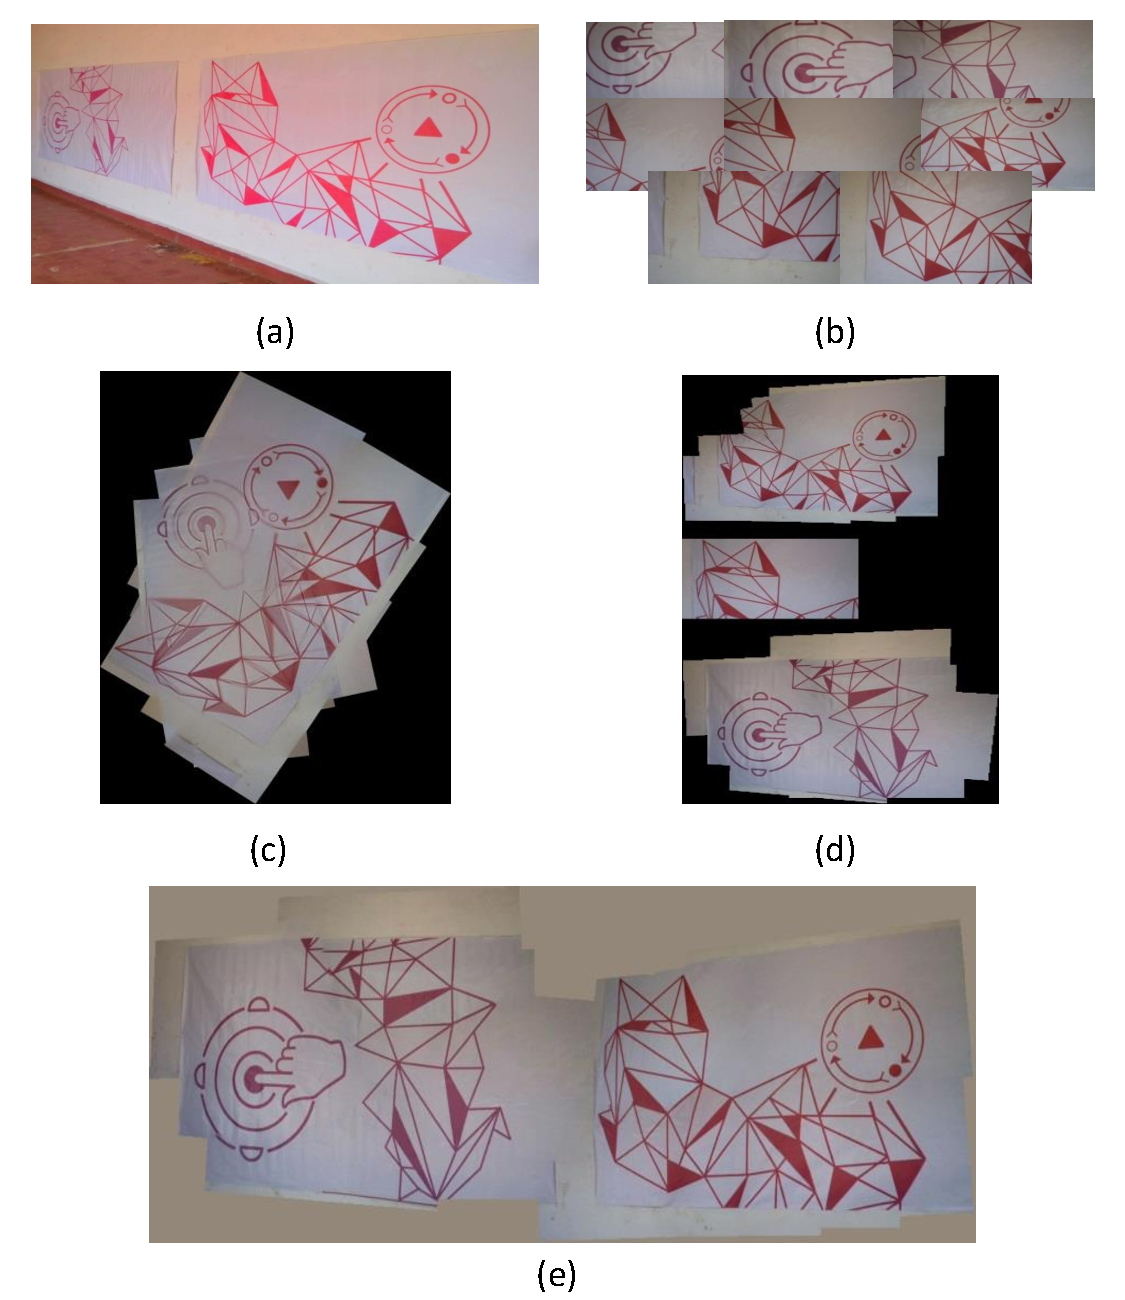
\includegraphics[width=0.85\linewidth]{mosaicing/results/Purple_red}
\caption{(a) An outdoor scene captured by a standard camera in an
  exhibition. Notice a significant gap between the two posters.  (b) Pruned
  images from the quadcopter video using our saliency algorithm. (c) Output of
  Autostitch~\cite{autostitch} on the selected images. The mosaic is not
  reasonable presumably because of the confusion in features. (d) Output of Adobe
  Photoshop CS6~\cite{photoshop} on the selected images. The vacant space posed a
  problem to the feature matching algorithm, so instead of a mosaic,
  individual pieces were output as mini-panoramas (e) Our output on
  the selected images. We are able to join two posters (separated by
  vacant space) using IMU data.}
\label{fig:results2}
\end{figure}

\section{Planned Work in Mosaicing through Quadcopter}
In this section we will see planned advancements in mosaicing through
quadcopter.
\subsection{Path Planning of Quadcopter}
\label{sec:furtherWork}
We encountered following problems while controlling quadcopter manually:
\begin{itemize}
  \item As manual control is not smooth, the most of the captured images are
  blurred.
  \item Coverage (area covered in unit time) is not uniform. 
  \item We may not be able to cover desired area completely (and exactly) due to
  manual errors.
\end{itemize}
So, the solution for these problems is planning the trajectory of the quadcopter
in order to ``cover'' the desired area. To achieve this, we have started
developing a tool based on PTAM (Parallel Tracking and Mapping).
Following work is done till date.

\textbf{UI :-} User may click points to define area he/she wants to cover on
planar region. Keypoints which are closest to clicked points are found and 2D convex
hull of those keypoints is shown to user for confirmation. User may add/remove
points; accordingly updated 2D convex hull will be shown.
		
\textbf{Path Planning :-} Once user confirms the area to cover, plane
equation is found using the keypoints inside 2D convex hull. Later, corners of
2D convex hull are projected on the calculated plane. Now, grid of overlapping
cells (fifty percent overlap in horizontal as well as vertical direction) is
formed inside the area formed by projected corners of convex hull, as shown in
Figure \ref{fig:pathPlanning}. Currently, width and height of each cell is fixed
but can be taken from user in future.

\begin{figure}[h!]
\centering
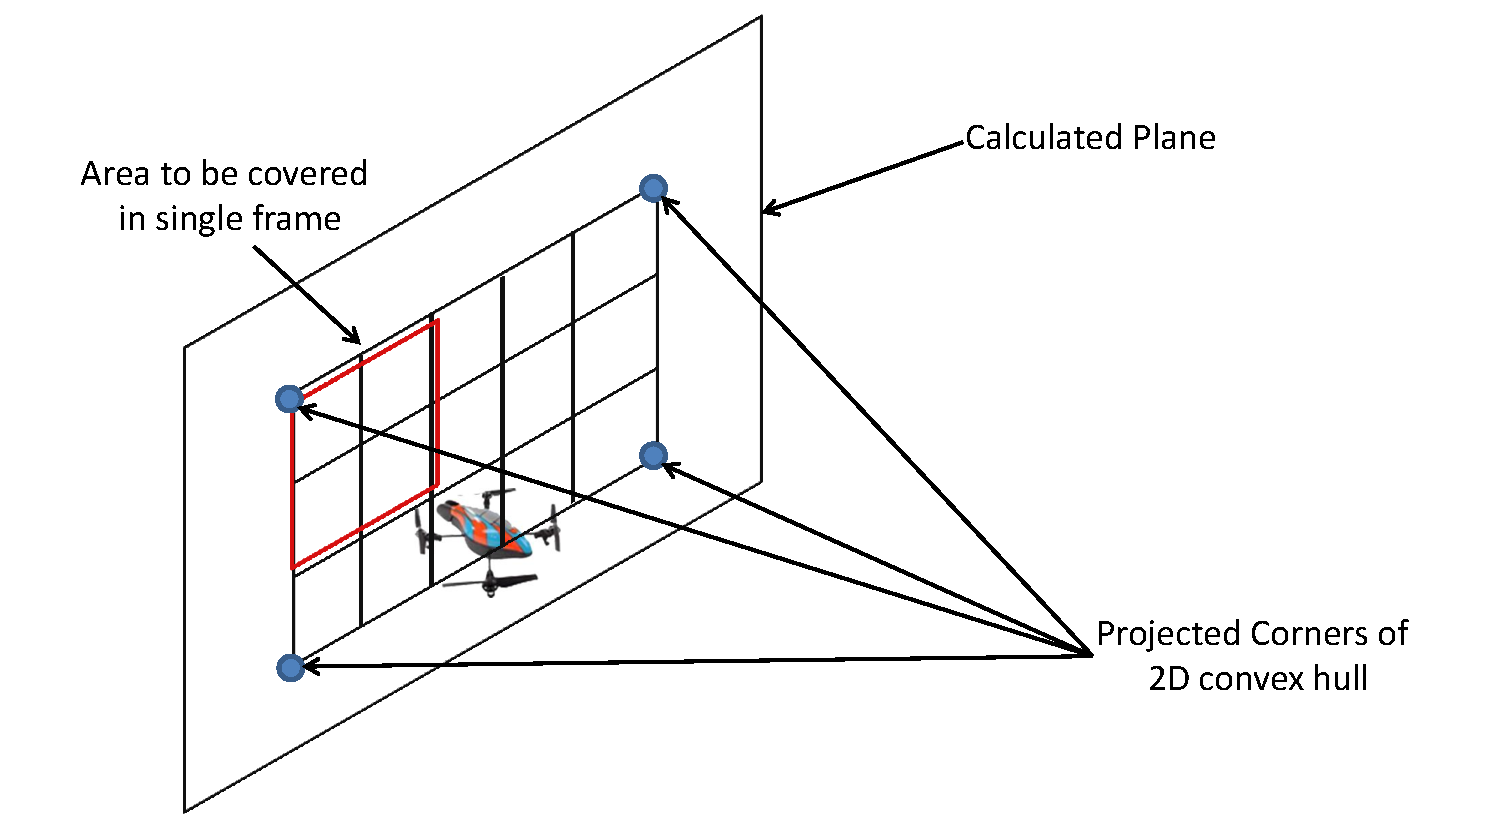
\includegraphics[width=\linewidth]{furtherWork/pathPlanning}
\caption{Schematic of path planning of quadcopter for single plane.}
\label{fig:pathPlanning}
\end{figure}

Basically, each cell in a grid represents area to covered in single frame.
Finally, camera extrinsics i.e., camera position is calculated for each cell in
the grid such that area in that cell will be covered in one frame. Accordingly,
quadcopter position is calculated for each calculated camera position.

Then, we maneuver quadcopter along the estimated trajectory and record
photographs at specified points.

\textbf{Further Work :-} We need to analyze the quality of images recorded at
specified points in order to find its usefulness for mosaicing. Accordingly we
may have to adapt path planning algorithm. 

\subsection{Multi-planar Cases}
In some cases, our area to be covered is actually divided in multiple planes
which are parallel to each other, but at different depths (e.g., poster boards
kept at different depths). So, instead of fitting single plane, we need to fit multiple
planes and repeat process (from grid formation) for each plane.

There may be some case where multiple planes will be at certain angle with each
other. There might be two subcases: one in which quadcopter is surrounded by
multiple planes (Figure \ref{fig:pathInnerOuter}:Left); second in which
quadcopter has to surround multiple planes (Figure \ref{fig:pathInnerOuter}:Right).
In both cases, we will cover individual planes as in the base case.  In the
first case, quadcopter will first rotate around its Z-axis before approaching
second plane. In the second case, quadcopter will move in circular trajectory
while moving from one plane to another plane. The control strategies for this
case is more complicated.

\begin{figure}[h!]
\centering
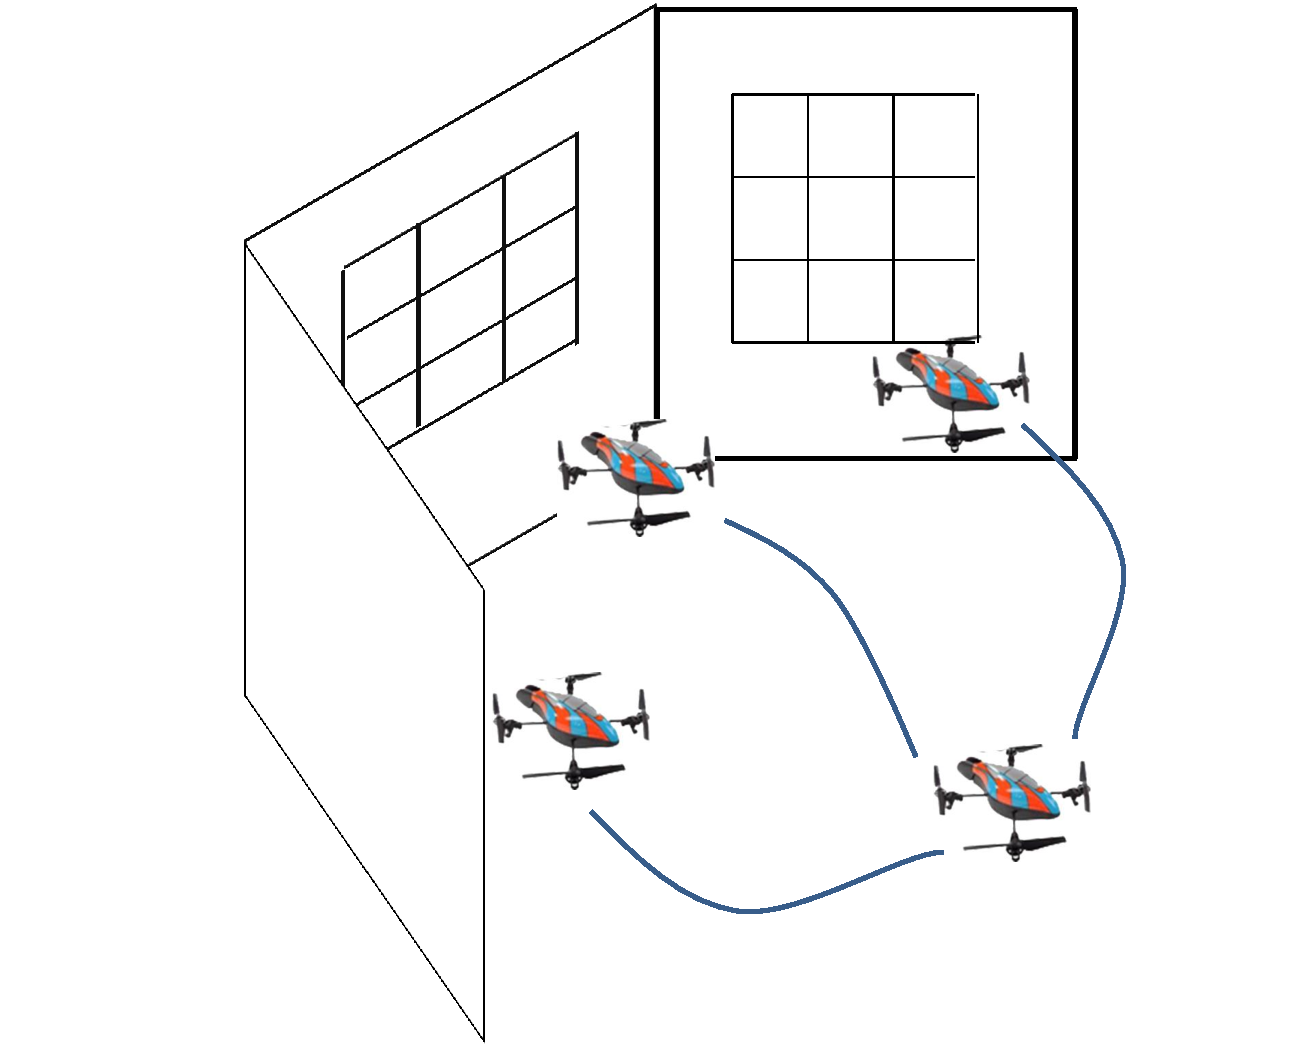
\includegraphics[width=0.45\linewidth]{furtherWork/pathInner}
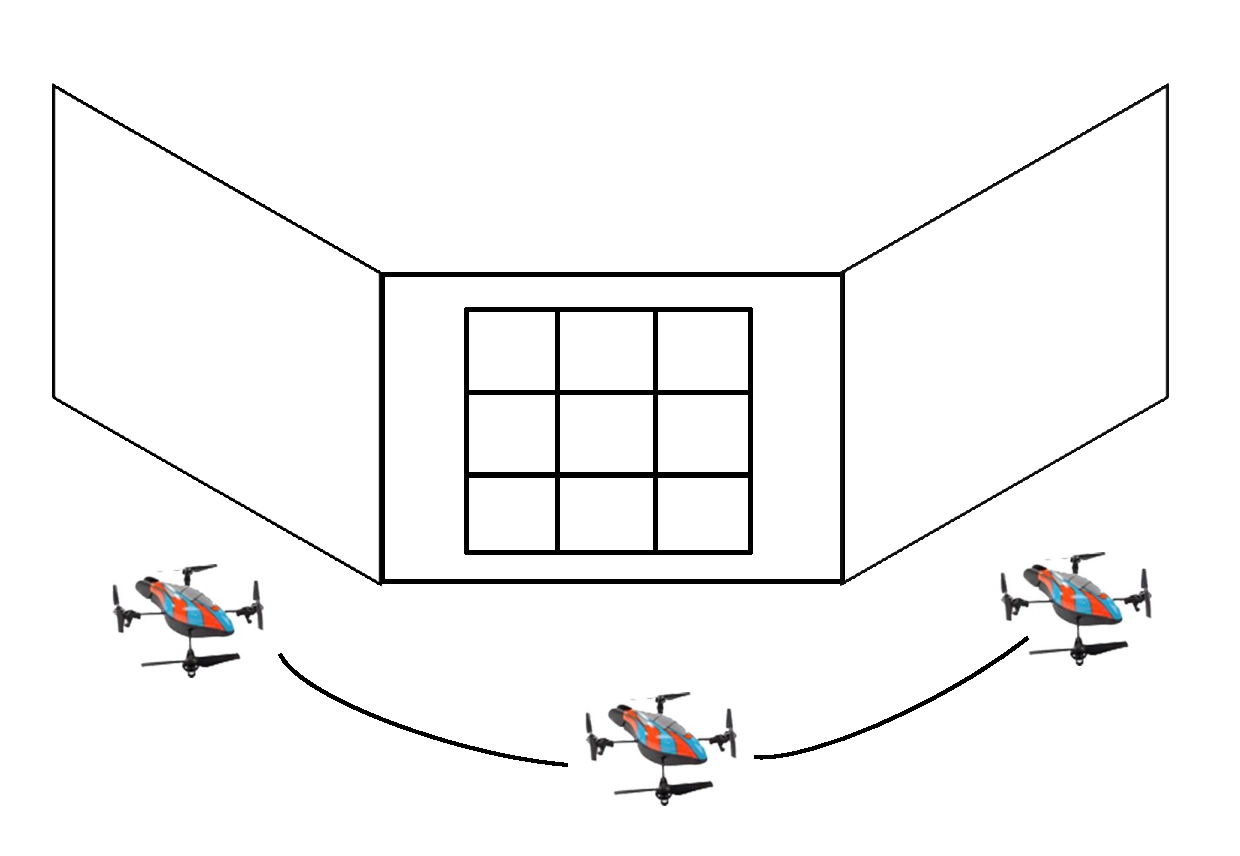
\includegraphics[width=0.45\linewidth]{furtherWork/pathOuter}
\caption{Schematic of path planning of quadcopter for multi-planar
cases.\textbf{Left:} Quadcopter is surrounded by multiple planes. 
\textbf{Right:} Quadcopter has to surround multiple planes.}
\label{fig:pathInnerOuter}
\end{figure}

\section{Quadcopter-based Stagnant Water Identification}

Dengue~\cite{WHO15Dengue} is a troublesome debilating disease with no
known preventing vaccine, or cure. Doctors advocate that the best way
to avoid this disease is to avoid being bitten by mosquitoes which is
virtually an impossibility for many people in India.  The greatest
risk of contracting dengue (pronounced DENgee) is in the Indian
subcontinent.  

Technology is a must in tackling this situation.  The risk of disease
can be reduced by using insect repellents. In our institute, the
common method has been the spraying of insecticides.  Reports in the
media~\cite{china} indicate that China has flooded a small island
releasing half a million sterile mosquitoes to dominate the potent
mosquitoes. Such measures have unknown and unforeseen environmental
impact on the eco-system. Regardless, researchers are convinced that
there is no one single magic bullet to tackle the disease. 

Our work, started prior to the announcement of ``Project
Premonition,'' is similar to that of \cite{Microsoft15}.  Instead of
attempting to destroy the mosquito, we seek to detect the reason for
the increased outbreak, especially in urban areas.  Our work complements that
of \cite{Microsoft15} --- the goal in \cite{Microsoft15} is to ``catch wild
mosquitoes'' (typically in the outfield) by creating novel mosquito traps, and
then to test mosquitoes for pathogens. New traps are placed by drones, and
retrieved by drones. In contrast, our work emphasizes the need for
identifying the location of these traps.  

\begin{figure}[h!]
\centering
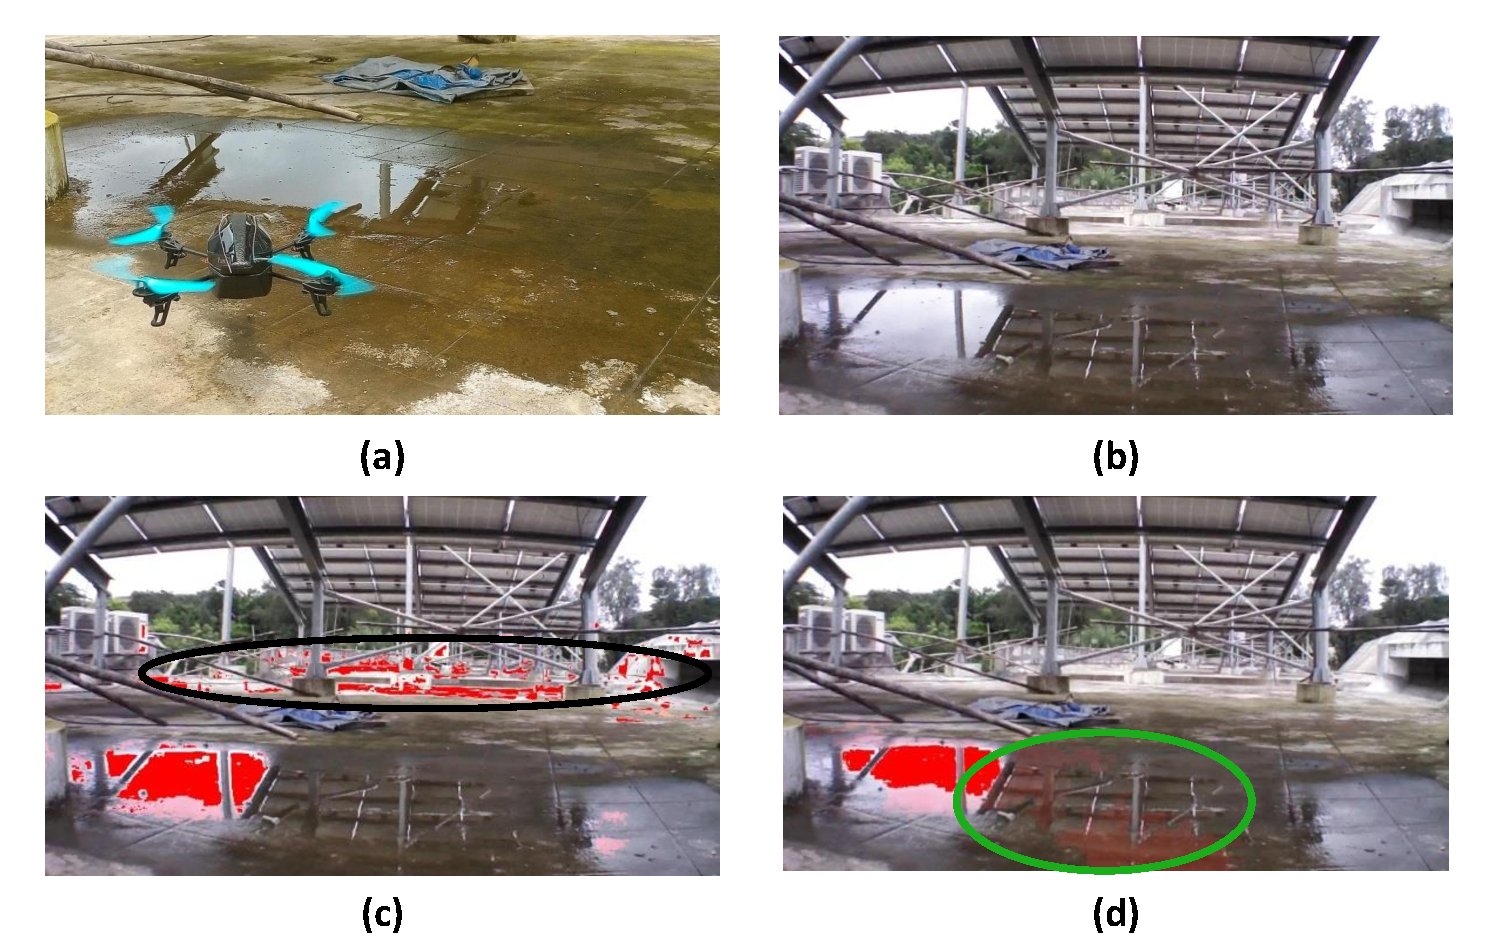
\includegraphics[width=\linewidth]{stagnantWater/figures/teaser.pdf}
\caption{(a) Our hovering quadcopter (b) A typical
  rooftop on campus (c) Earlier method \cite{rankin2004daytime} applied, and
  output marked in red (d) Our output. Notice (marked as black oval in
  (c)) that \cite{rankin2004daytime} confuses non-puddle patches as puddle.
  Also, note (marked as green ellipse in (d)) that \cite{rankin2004daytime} is
  not able to detect puddle which are dark.}
\label{teaser} 
\end{figure}

One of the major reasons behind the growth of mosquitoes is the
continuous existence of \emph{water puddles} around residencies in
urban India.  The virus is carried by mosquitoes, and these breed in
stagnant water. \emph{Can we detect stagnant water?}  When we surveyed
terraces (Fig.~\ref{teaser}) and ``chajjas'' of various buildings in
our institute, we found split AC air conditioners dumping condensed
water. Such areas can be surveyed using autonomous quadcopters.

\subsection{Related Work}
The method in ~\cite{santana12} for detection of
water relies on the chaotic nature of water's dynamic texture to
exploit a measure of entropy over the trajectories obtained from
optical flow trackers over several frames. \cite{zhang10} has
introduced a descriptor which is tolerant to the flip transformation
and even non-rigid distortions, such as ripple effects.  \emph{These
  methods and others in the literature focus on the turbulent aspects
  of water}, largely absent in our application that focuses on
stagnant water.  Our method is closest to that of Rankin et
al.~\cite{rankin2004daytime, rankin11} who have implemented a rule-based water
detector based on sky reflections.  These rules are established
based on an analysis of images captured in wide-open areas on
cross-country terrain. Not only do we have new methods, \emph{our
datasets are captured in urban areas using a quadcopter and thus these
rules seem unlikely to be readily applicable.}

\subsection{Methodology}
Our method is based on a combination of color based method with an optical flow
based method.  We establish the need for the combination in the first two subsections.
\vspace{0.5cm}
\noindent\textbf{Appearance-based Detection}

\begin{figure}[h!]
  \centering
  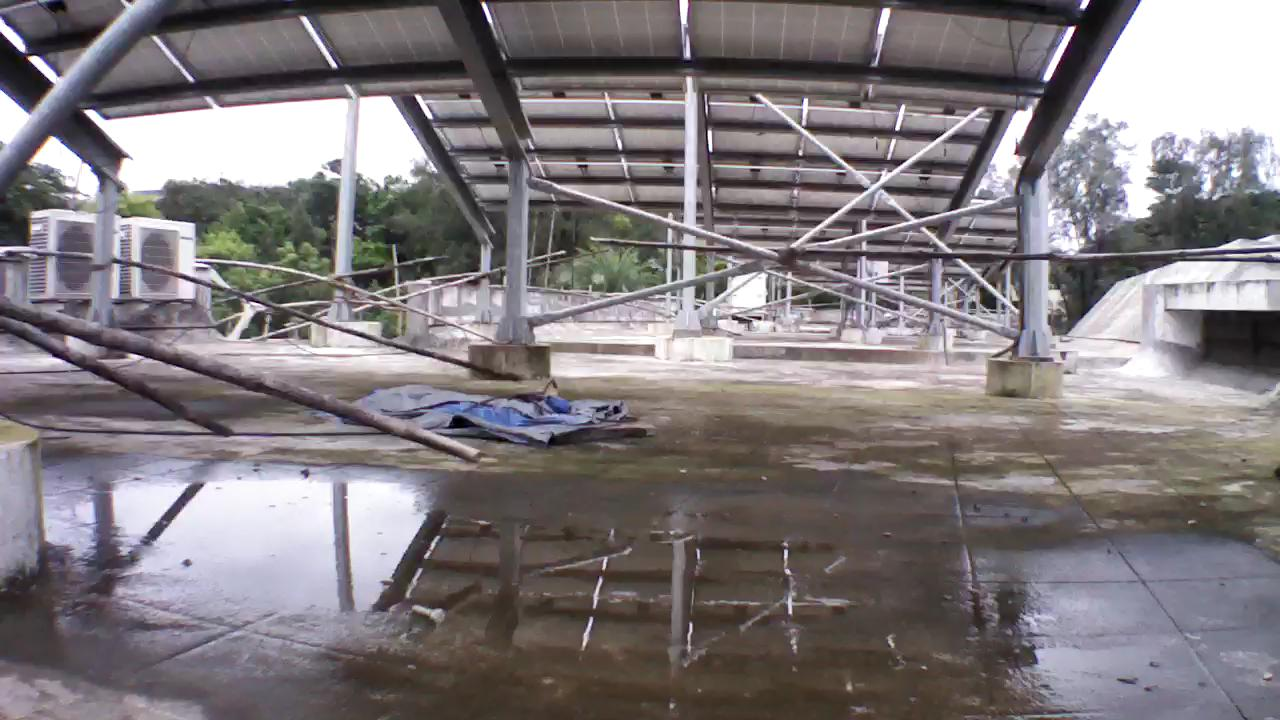
\includegraphics[width=0.4\linewidth]{stagnantWater/figures/IMG_PAIR_27_1}
  \hfill
  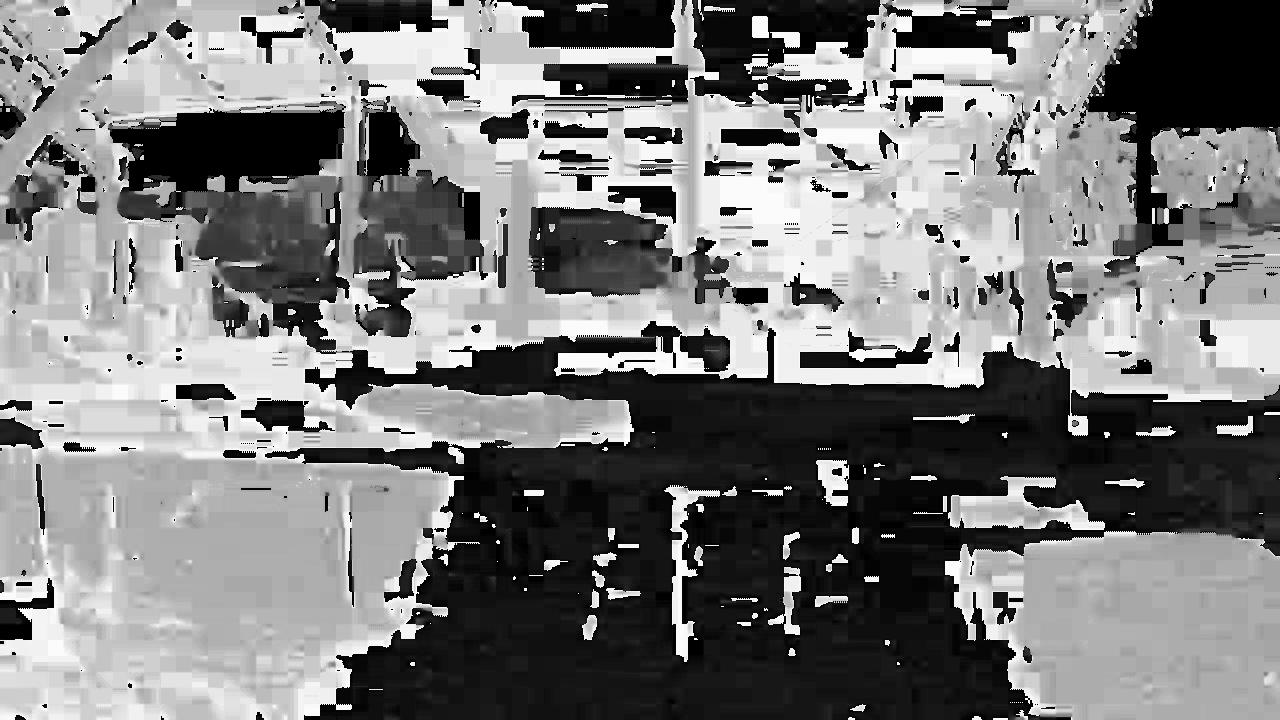
\includegraphics[width=0.4\linewidth]{stagnantWater/figures/IMG_PAIR_27_1_H} 

  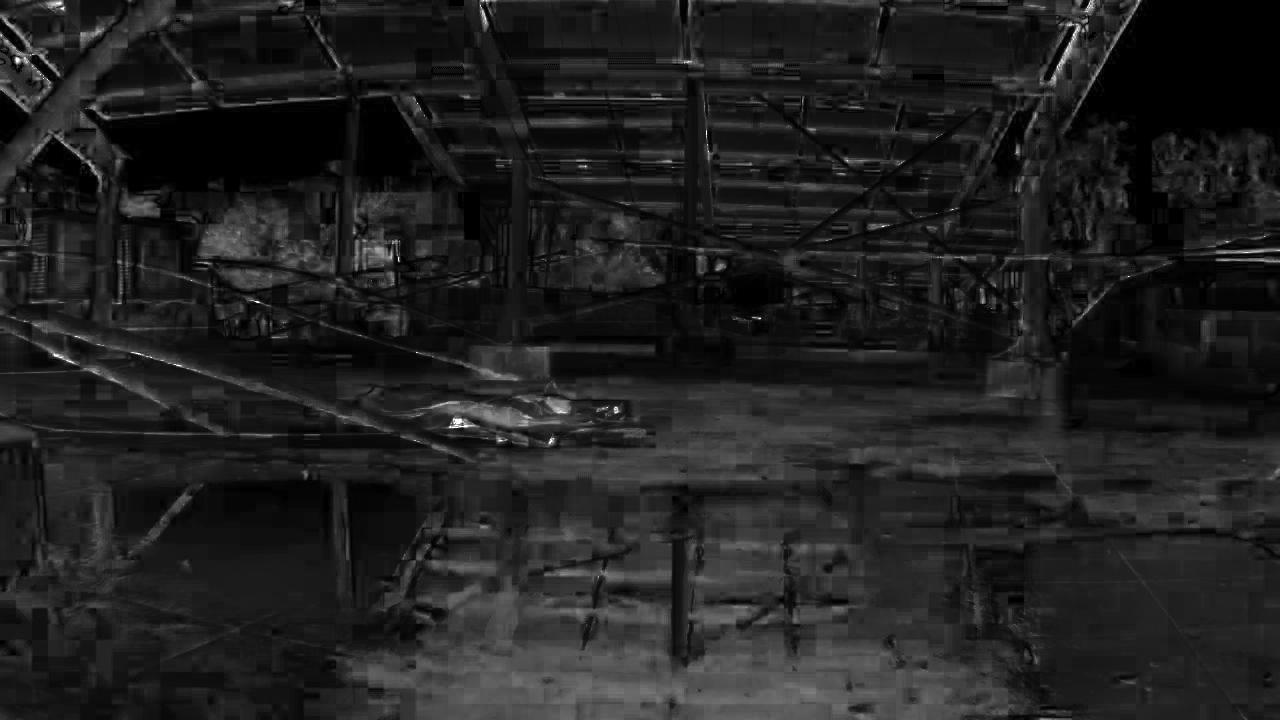
\includegraphics[width=0.4\linewidth]{stagnantWater/figures/IMG_PAIR_27_1_S}
  \hfill
  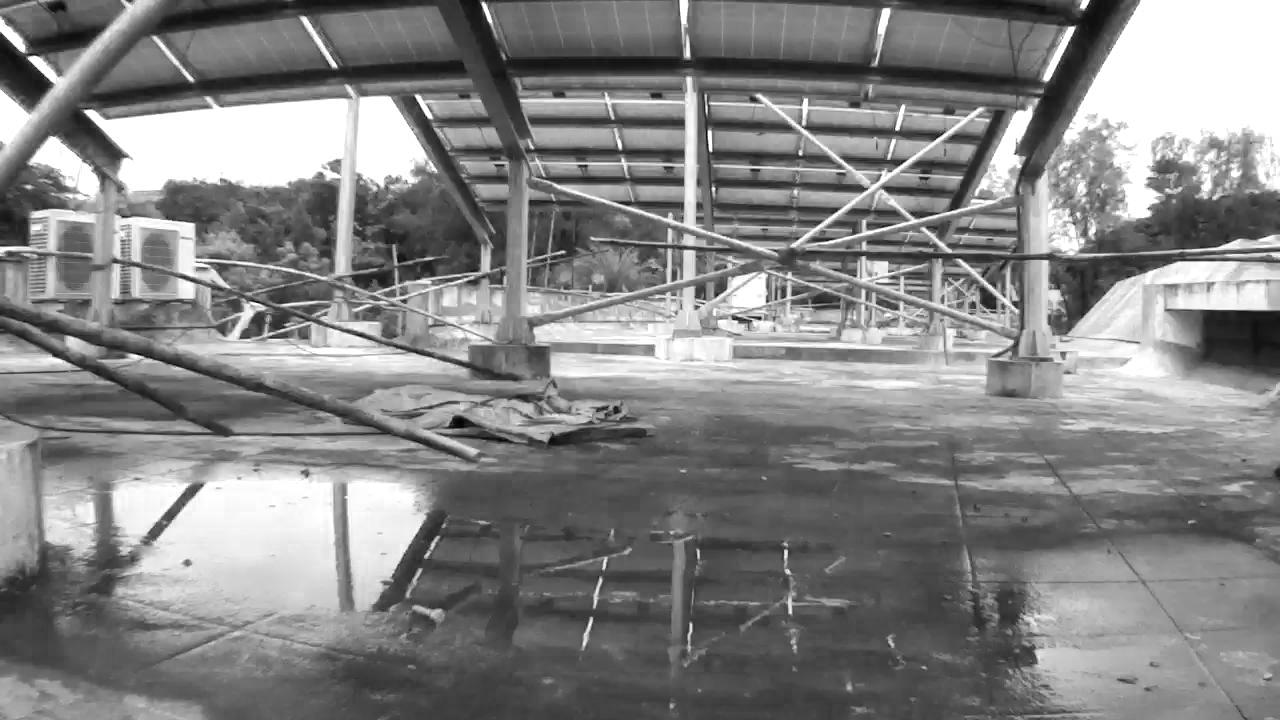
\includegraphics[width=0.4\linewidth]{stagnantWater/figures/IMG_PAIR_27_1_V}
  \caption{An image (top left) and the HSV components.  The puddle has
    low saturation (bottom left) but high intensity (bottom right).
    The hue is indeterminable and is based on the environment.}
  \label{fig:HSV}
\end{figure}

Under ambient lighting conditions, puddle areas display high
brightness and low saturation as can be seen in
Fig.~\ref{fig:HSV}. Features based on these are fed to an SVM
classifier. Training an SVM is a labour intensive task.  To reduce the
effort, we have developed a tool shown in Fig.~\ref{fig:training}. 

\begin{figure}[h!]
  \centering
  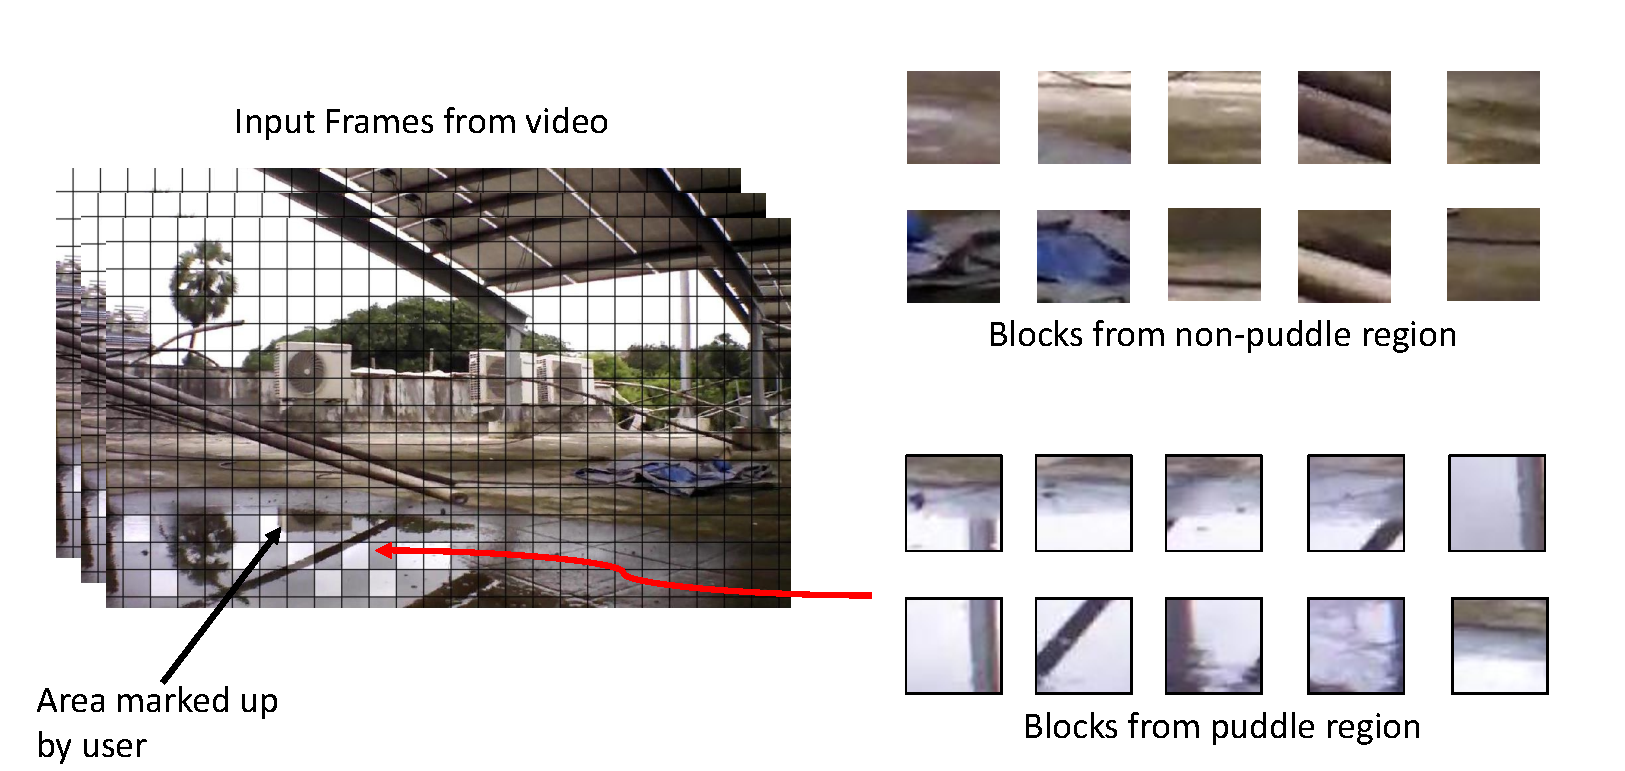
\includegraphics[width=0.9\linewidth]{stagnantWater/figures/trainingData.pdf}
  \caption{The process for creation of training data. The user selects
    the stagnant water area by drawing a contour to produce `positive'
    and `negative'  data.}
  \label{fig:training}
\end{figure}

\textbf{Failure of SVM-based methods:} The SVM detector is good at
detecting regions of sky reflected off a puddle.  In the HSV color
space, these regions have low saturation (S) and high brightness (V)
values, and are picked up with high reliability by the HSV histogram
feature based SVM detector. However, false negatives are also produced
since other reflected regions such as trees, buildings, etc. are
usually classified as non-puddle regions as many of these
characteristics is shared by negative images in the training data set.
\vspace{0.5cm}

\noindent\textbf{Optical flow based Detection}
Fortunately our images are captured by a moving quadcopter.  The
optical flow measures apparent motion of objects in a scene caused by
relative motion between camera and object. The magnitude of the
optical flow is high for objects that are close in comparison to
objects at a distance.  Fig.~\ref{fig:optical_flow} shows the
magnitude of optical flow calculated from two images.

\begin{figure}[h!]
  \centering
  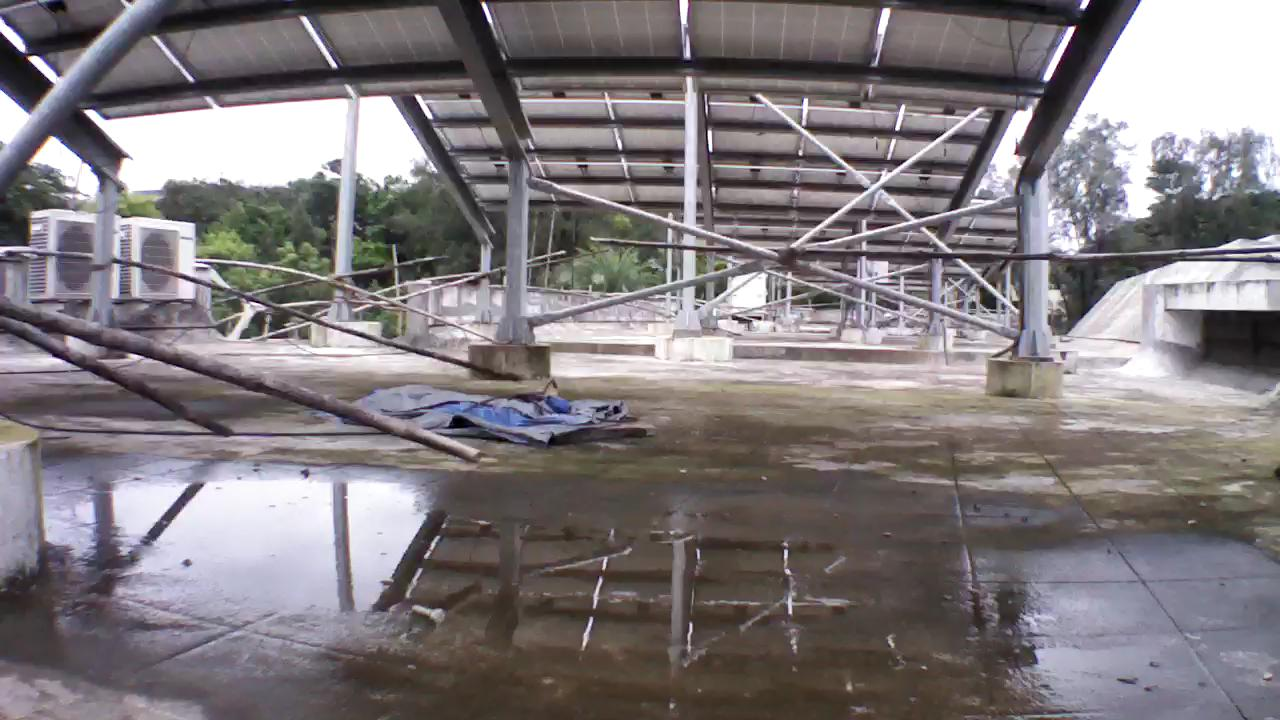
\includegraphics[width=0.32\linewidth]{stagnantWater/figures/IMG_PAIR_27_1}
  \hfill
  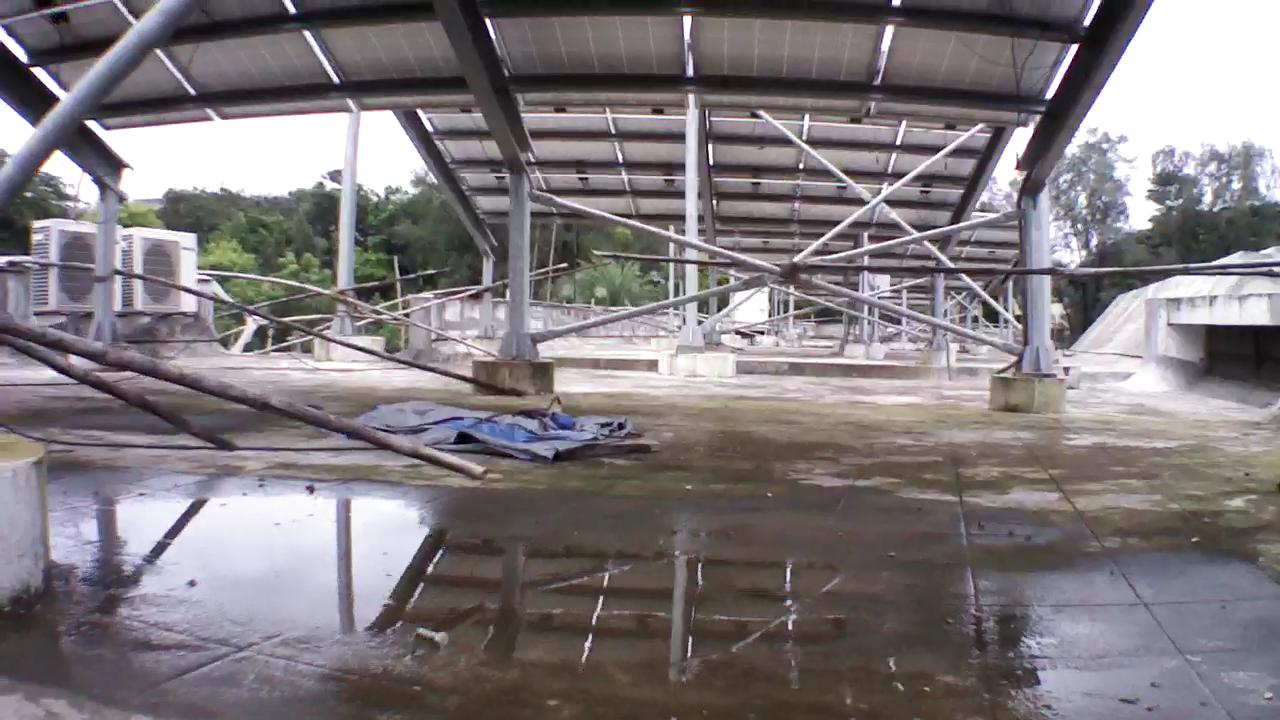
\includegraphics[width=0.32\linewidth]{stagnantWater/figures/IMG_PAIR_27_2}
  \hfill
  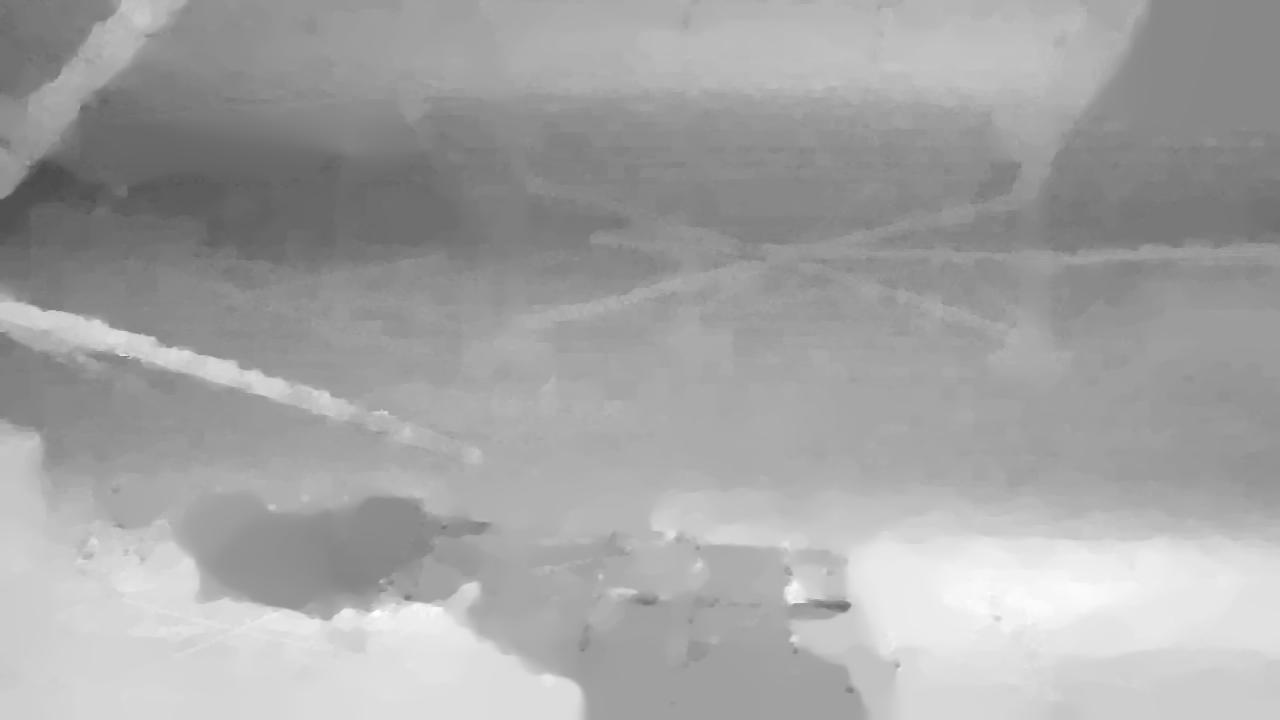
\includegraphics[width=0.32\linewidth]{stagnantWater/figures/IMG_PAIR_27_optical_flow}
  \caption{Optical Flow. Left, Middle: Frames taken from positions
    which are $d$ units apart in 3D world. $ 0.01 \leq d \leq 0.1$. Right:
    Magnitude of optical flow. We observe that the magnitude of optical
    flow in the reflective parts of the puddle is relatively low.}
  \label{fig:optical_flow}
\end{figure}

A recent thesis \cite{Liu11Thesis} has one of the state of the art
algorithm for optical flow. One requirement is the need for
spatio-temporal smoothness constraint which can be challenging because
of the jerky movement of the UAV.  To resolve this, we use the
Inertial Measurement Unit (IMU) data available on the quadcopter to
synchronize positional information with the video sequence captured by
quadcopter. In short, we select the frame pair which are spatially the
closest, among a set of competing temporally adjacent frames.

\textbf{Failure of optical flow:} Optical flow is essentially being
used in a depth from parallax mode to exploit the fact that still
puddles behave like mirrors. The scenery reflected by such puddles is
usually at a much greater depth than the immediate surroundings of the
puddle.  Optical flow is largely independent of hue and saturation.
For the same reason, however, optical flow as a means of detecting
puddles will fail to report true positives when the object that is
being reflected is close by. In such cases, the saturation and
intensity values are useful.

Yet another reason for the failure for the optical flow is the
inability to distinguish true ``far away'' regions versus imagined far
away regions due to the mirror-like properties of water.  To handle
these false positives, we devise a horizon mask based on the principle
that water flows down.
\vspace{0.5cm}

\noindent\textbf{Combined approach}

\textbf{Horizon Mask:} The change in depth for far-away scenes as well
as their reflections on puddle, in consecutive frames, are hard to
distinguish. In previous work \cite{rankin11} such issues are avoided
by discarding a fixed-portion of image corresponding to far-off
regions, enforced by constrained input capture method. Due to
inapplicability of such constraints in the comparatively agile input
capture conditions of quadcopter, features derived from urban
environment are utilized for finding plausible puddle regions. In
urban setting, the high availability of structures in surroundings,
having distinctly flat surfaces and rectilinear silhouettes, enables
use of edge-detection based methods to bound planar regions that can
contain puddle. Applying the Hough transform with calibrated
parameters followed by length-based selection of lines detected, a
upper boundary for puddle region called `Horizon' is found. The
Horizon is in turn used to create a binary mask to be applied to local
scores from other techniques before normalization.

\begin{figure}[h!]
  \centering
  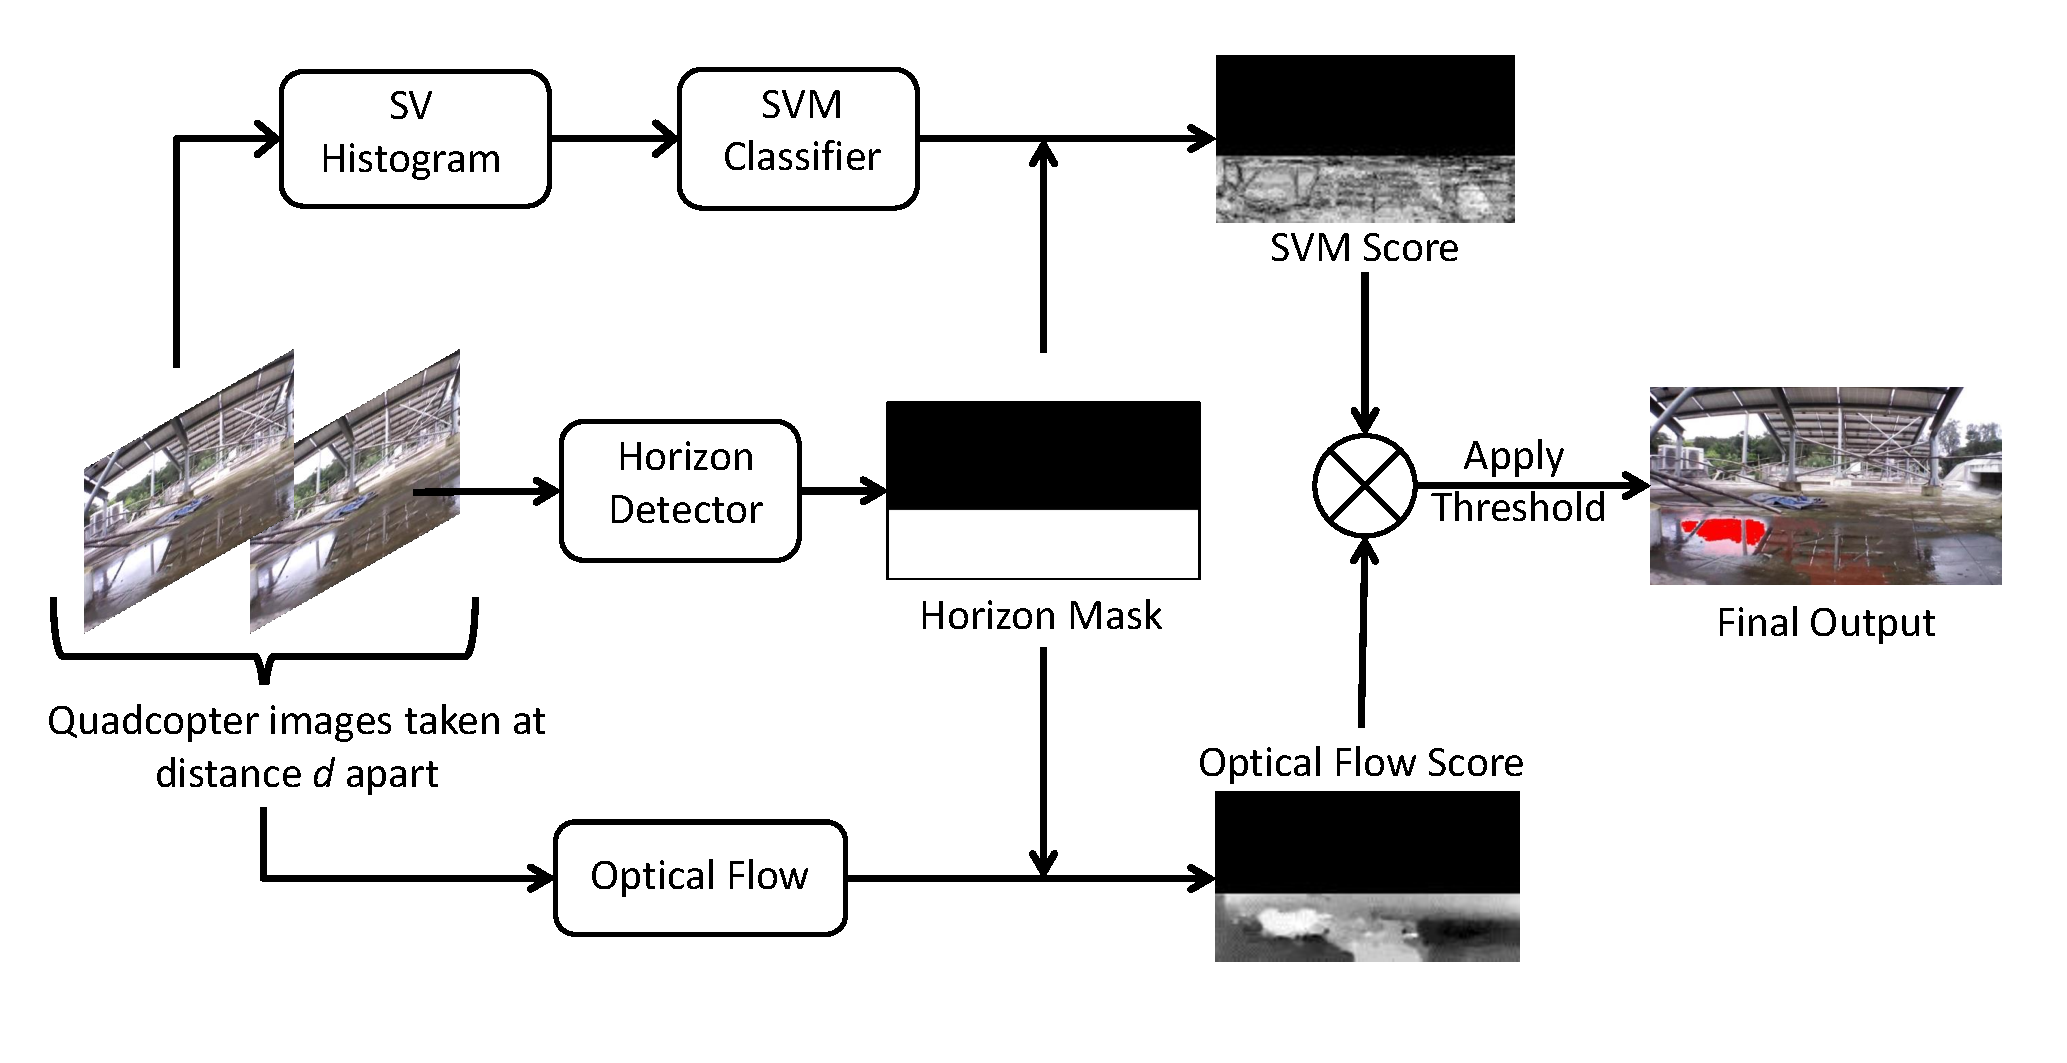
\includegraphics[width=\textwidth]{stagnantWater/figures/overall_workflow.pdf}
  \caption{Overall architecture.}
  \label{fig:workflow}
\end{figure}

These observations suggested a novel combined approach as sketched
in Fig.~\ref{fig:workflow}.

\subsection{Experiments and Results}

All our experiments have been completed with the inexpensive consumer
quadcopter called Parrot's AR Drone. We remark that one should not
compare expensive military grade drones with such inexpensive drones.
For the purpose of showing the efficacy of our method, we also took a
picture of the scene from a distance with a 5 mega-pixel camera for
the reader to better understand the scene.  We covered urban places
such as terraces, constructions sites, building backyards,
pumping stations, and so on.  We have captured around eight different
types of datasets, each having around two-three minutes of video
(around 3000 frames each). 

\textbf{Comparison:} We compare our method to \cite{rankin2004daytime} on
representative images since the methods in \cite{rankin11} do not apply. 
%See Fig.~\ref{fig:comparison}. 
It can be seen from Fig.~\ref{fig:comparison} that in all images,
\cite{rankin2004daytime} is confusing  bright patches as puddle patches (note
red patches on walls, sky etc. in middle column in Fig.~\ref{fig:comparison}).
Also, \cite{rankin2004daytime} is not able to detect textured puddle images (as
seen in the first row in Fig.~\ref{fig:comparison}). (The confidence in
detection is indicated by red hue in the output image. So, darker the red
tinge, higher the confidence in detected water region.)

\begin{figure}
  \centering
   
  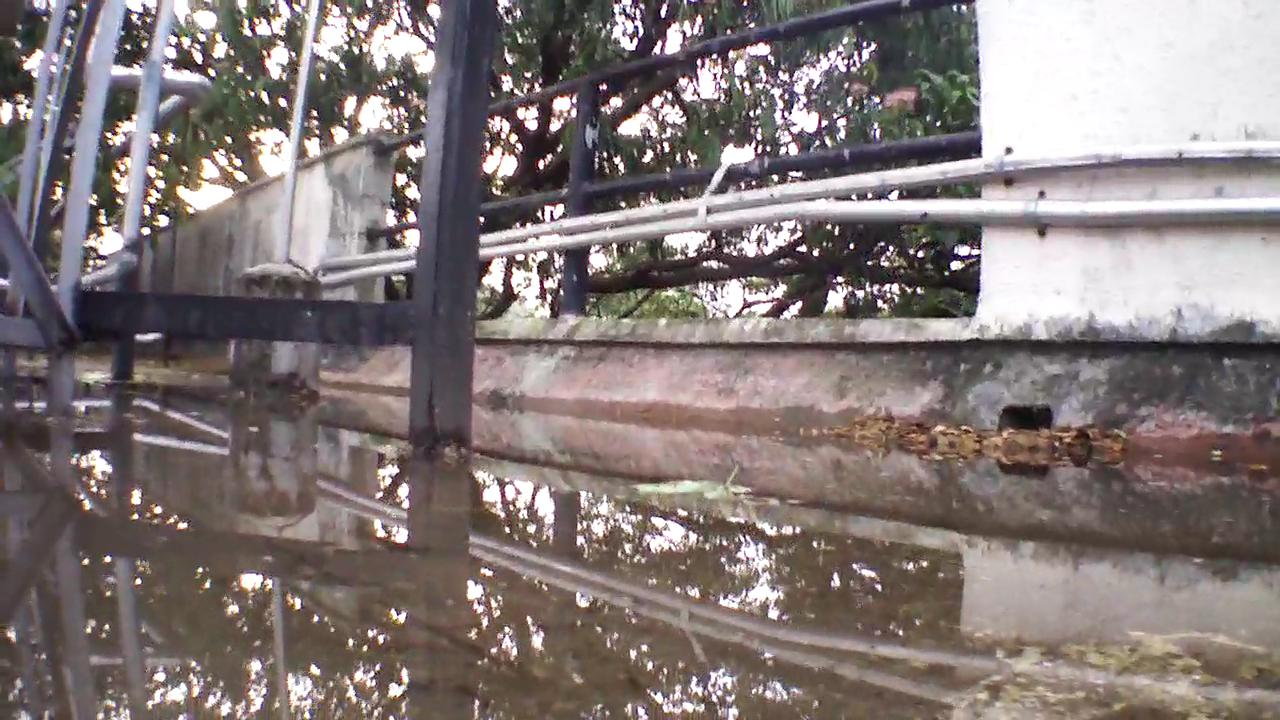
\includegraphics[width=0.32\linewidth]{stagnantWater/results/dataset_73/IMG_PAIR_124_1} \hfill
  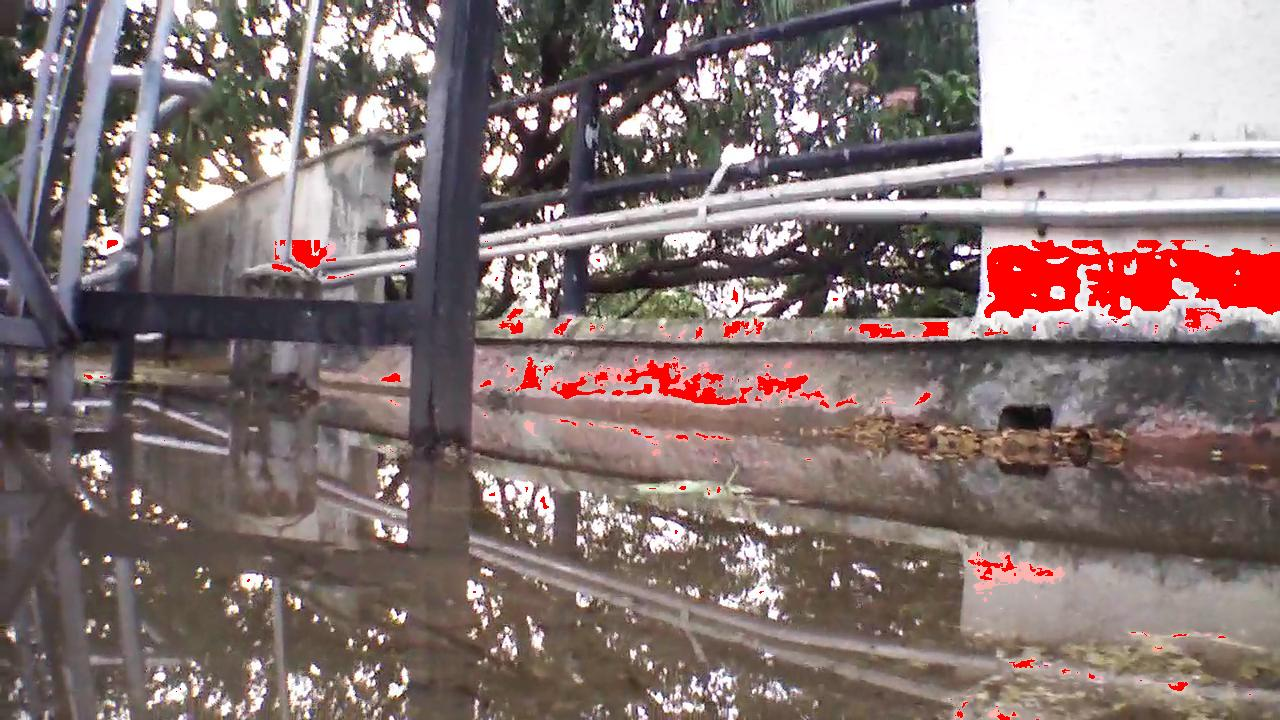
\includegraphics[width=0.32\linewidth]{stagnantWater/results/dataset_73/output_124_jpl2} \hfill
  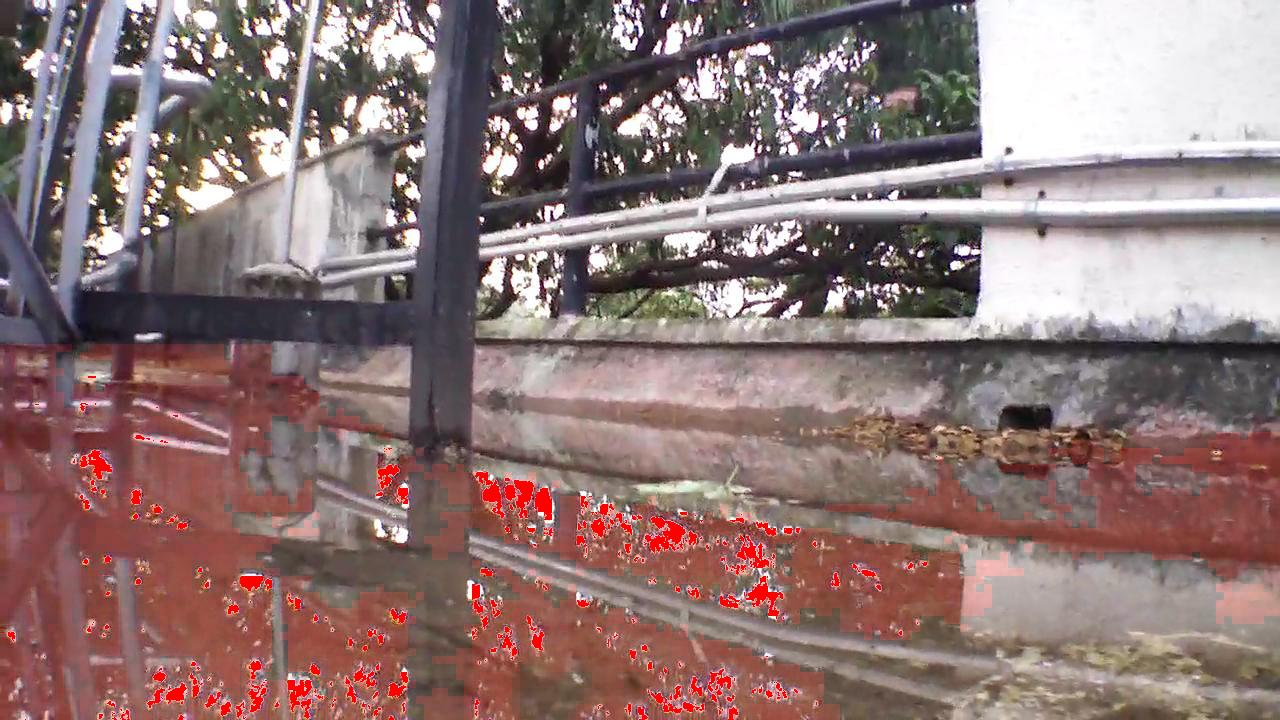
\includegraphics[width=0.32\linewidth]{stagnantWater/results/dataset_73/output_124}

  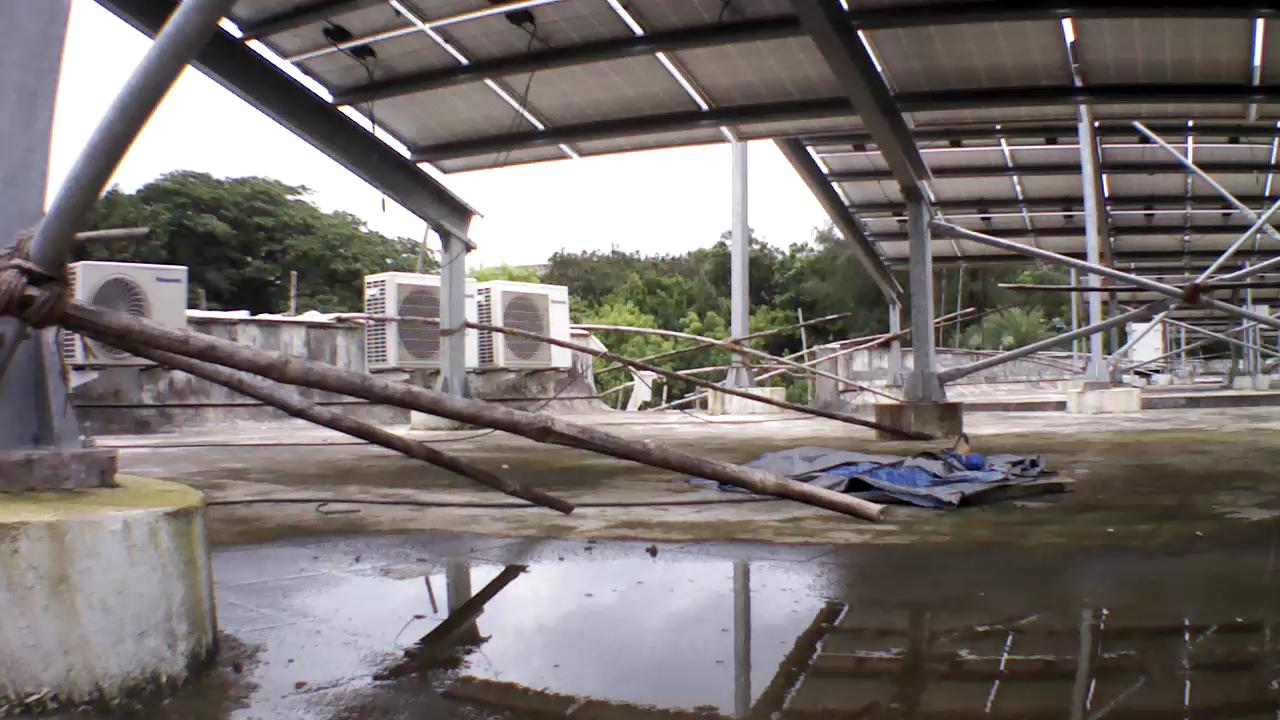
\includegraphics[width=0.32\linewidth]{stagnantWater/results/dataset_81/IMG_PAIR_1_1} \hfill
  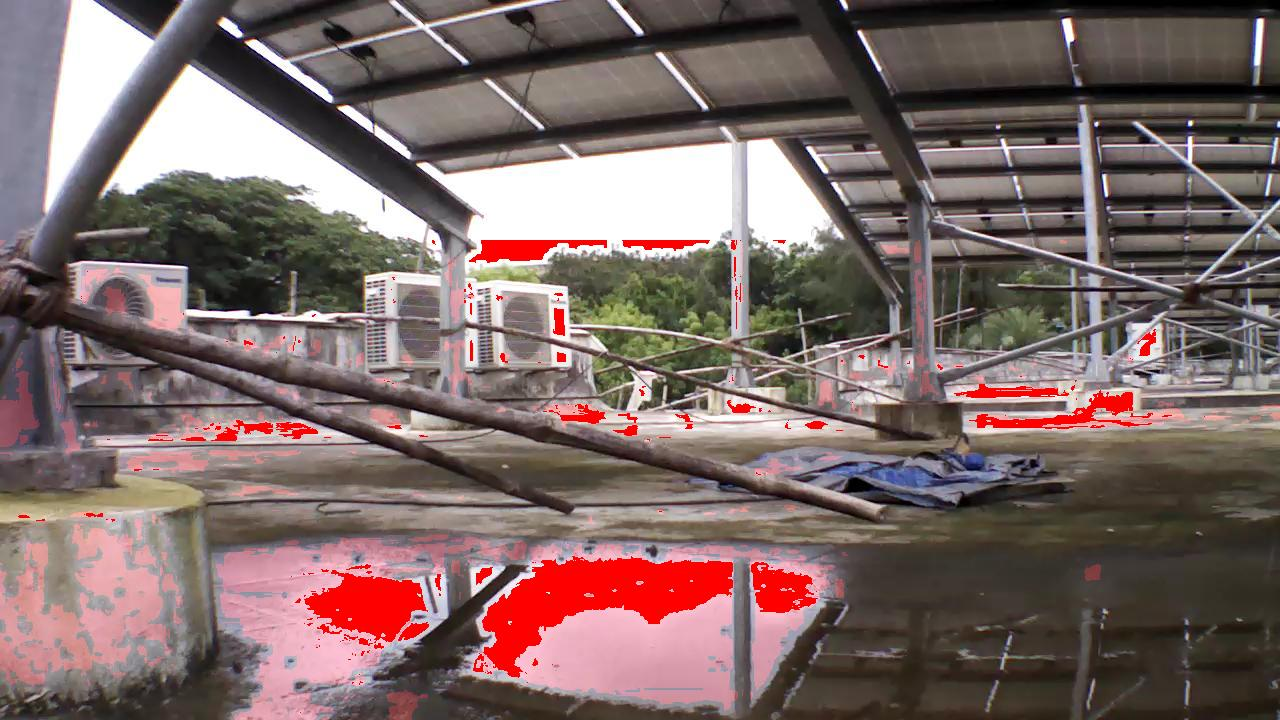
\includegraphics[width=0.32\linewidth]{stagnantWater/results/dataset_81/output_1_jpl2} \hfill
  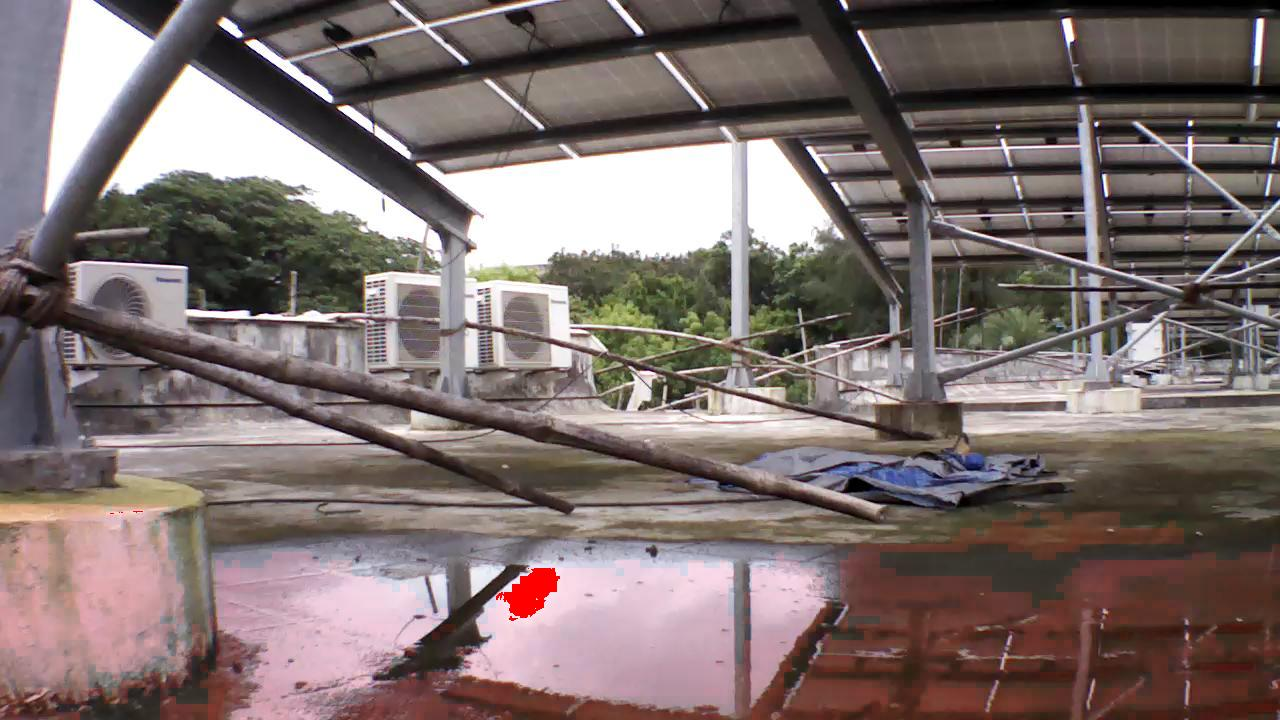
\includegraphics[width=0.32\linewidth]{stagnantWater/results/dataset_81/output_1}

  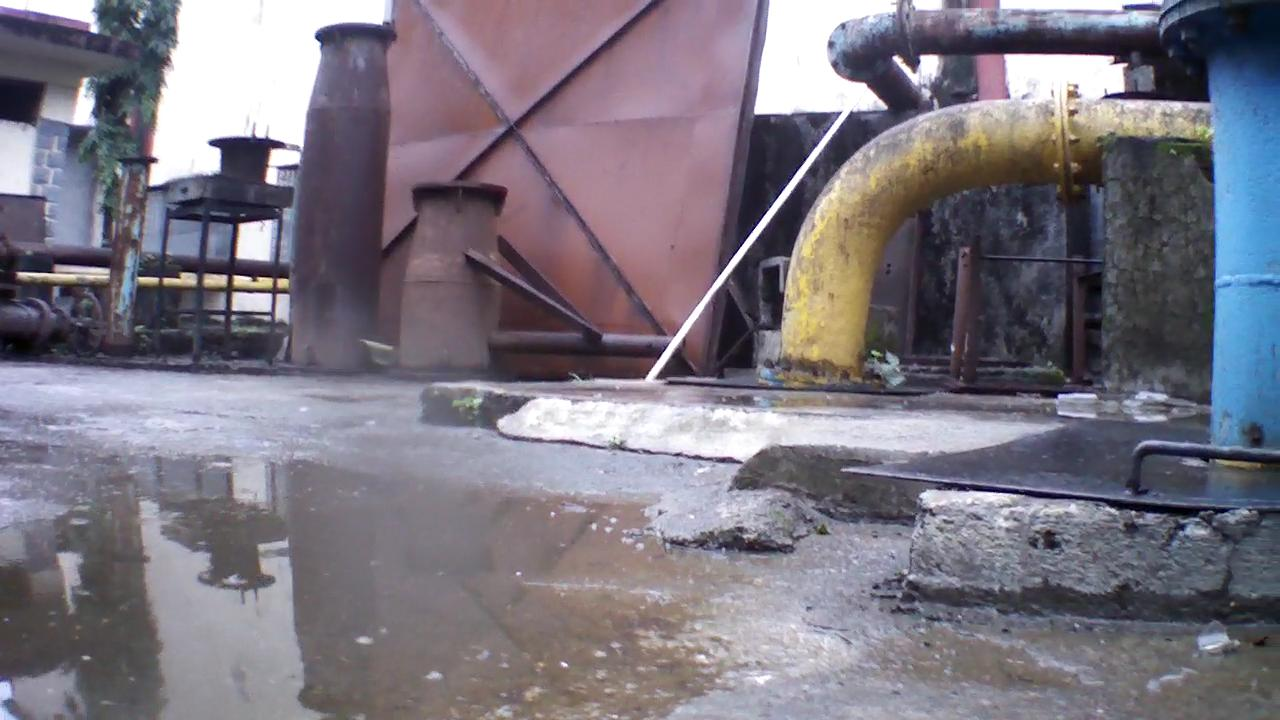
\includegraphics[width=0.32\linewidth]{stagnantWater/results/dataset_82/IMG_PAIR_192_1} \hfill
  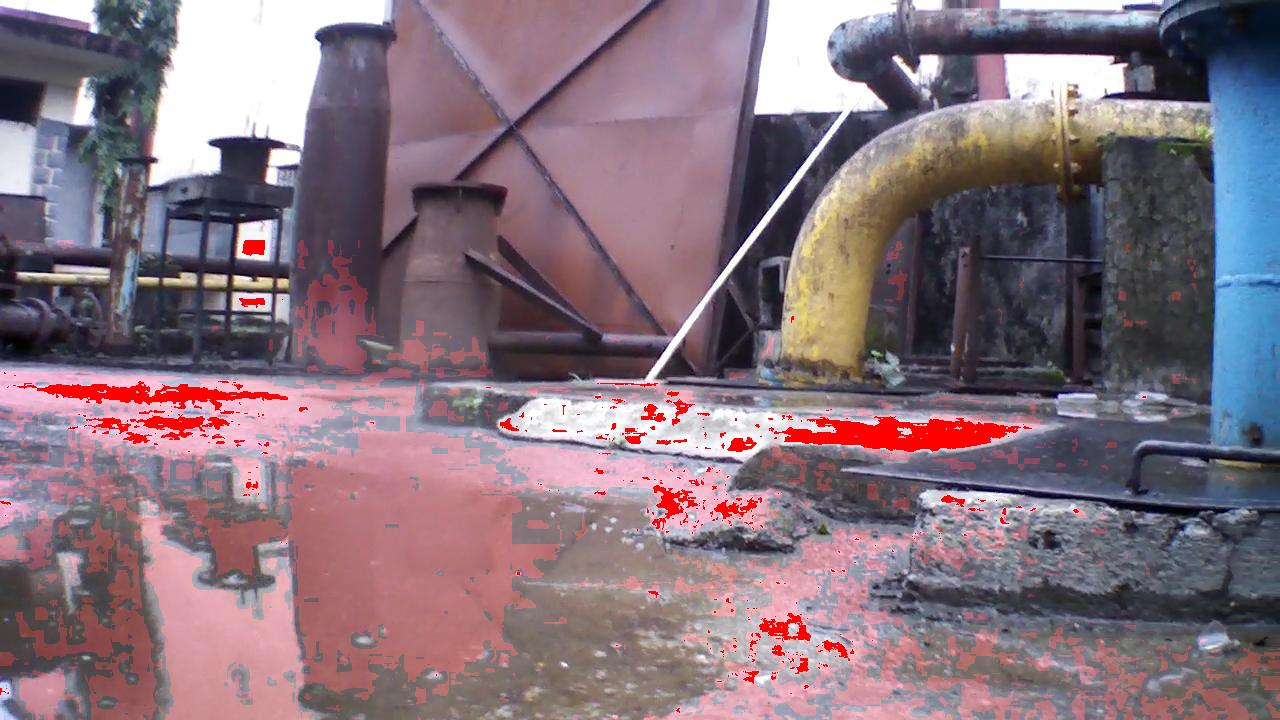
\includegraphics[width=0.32\linewidth]{stagnantWater/results/dataset_82/output_192_jpl2} \hfill
  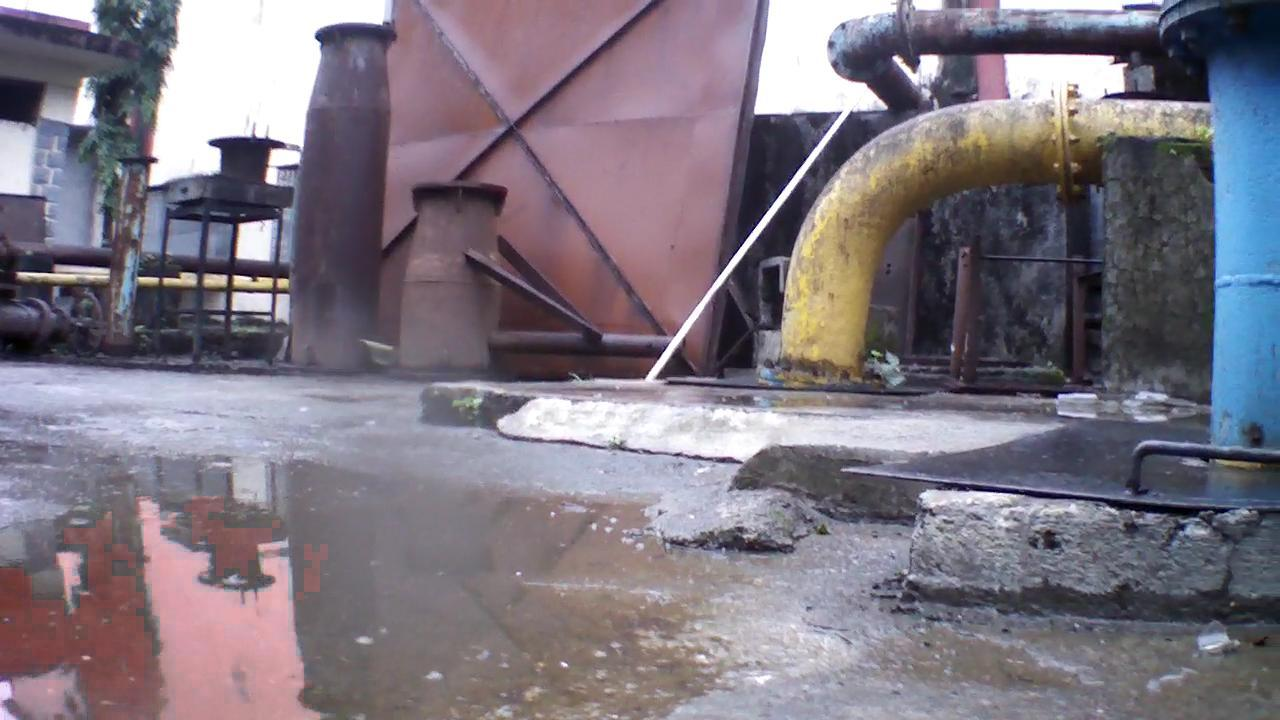
\includegraphics[width=0.32\linewidth]{stagnantWater/results/dataset_82/output_192}
  
  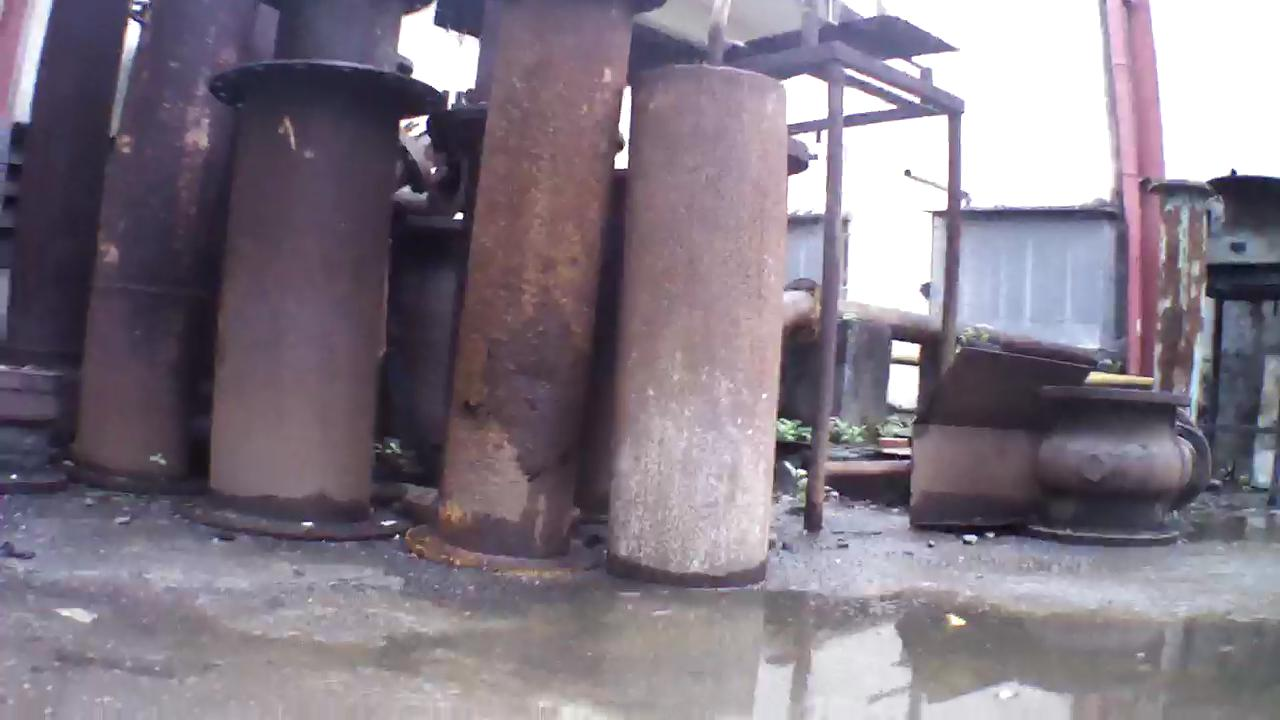
\includegraphics[width=0.32\linewidth]{stagnantWater/results/dataset_83/IMG_PAIR_130_1} \hfill
  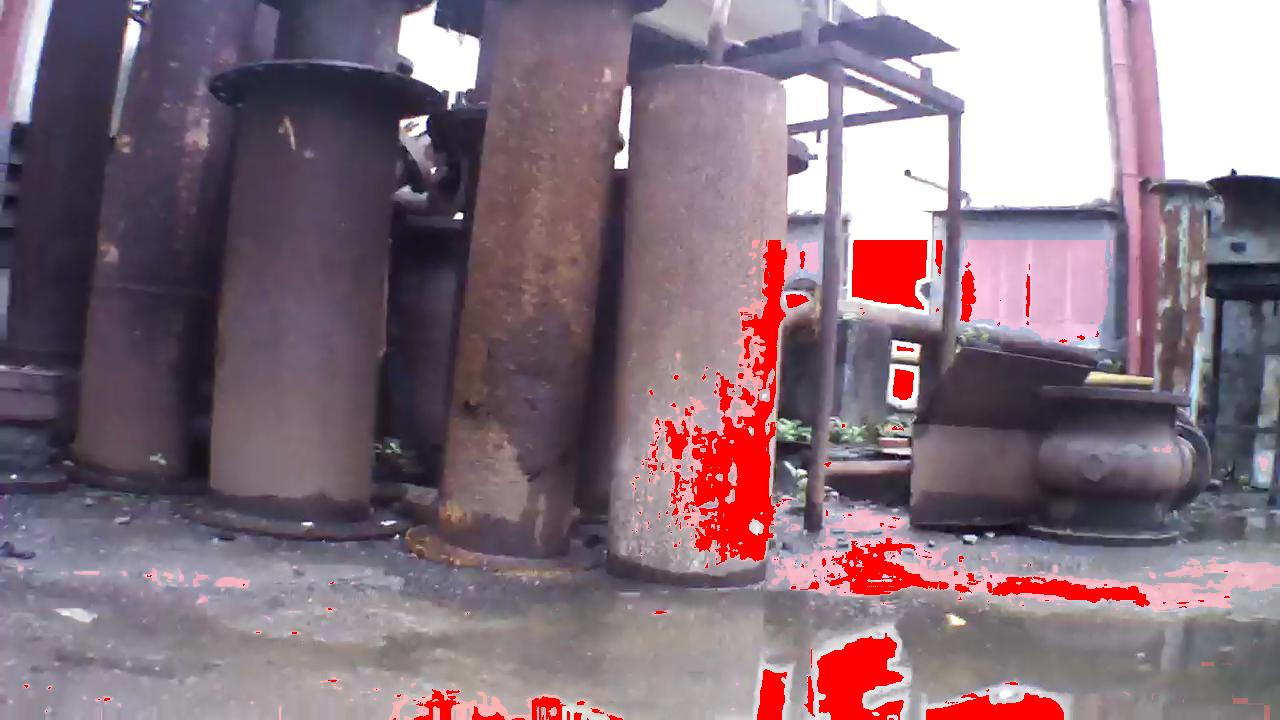
\includegraphics[width=0.32\linewidth]{stagnantWater/results/dataset_83/output_130_jpl2} \hfill
  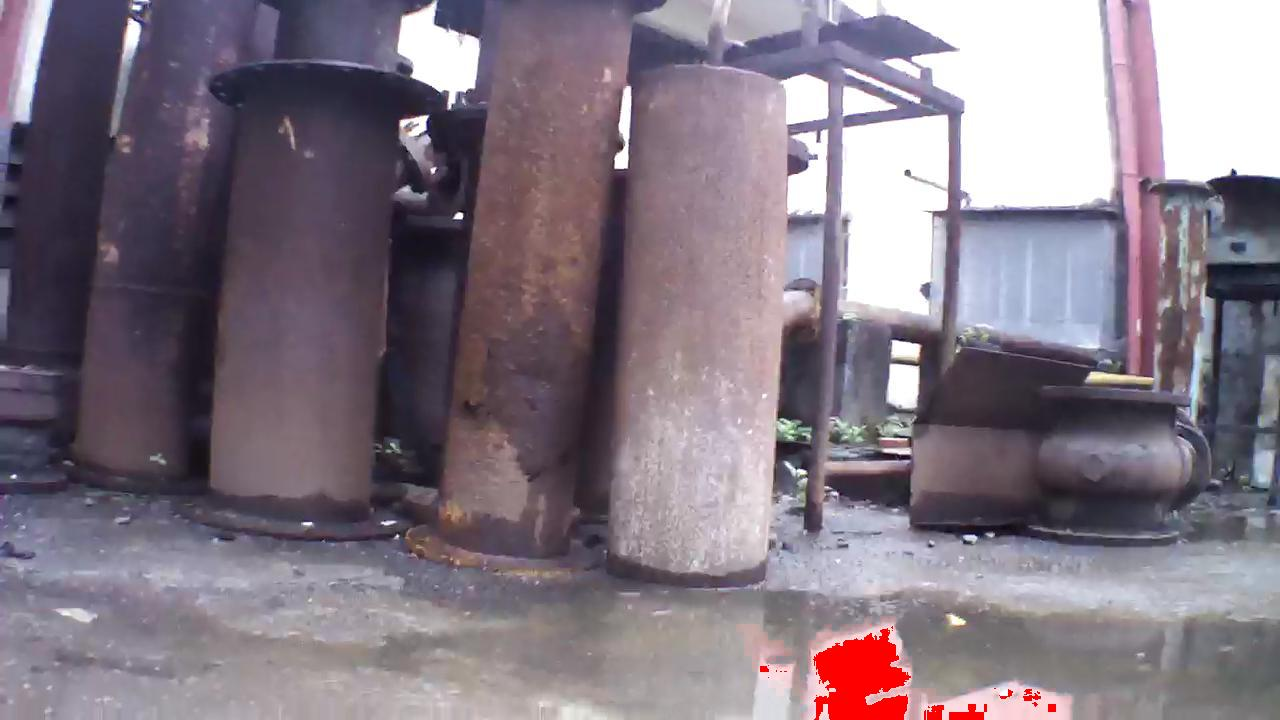
\includegraphics[width=0.32\linewidth]{stagnantWater/results/dataset_83/output_130}

  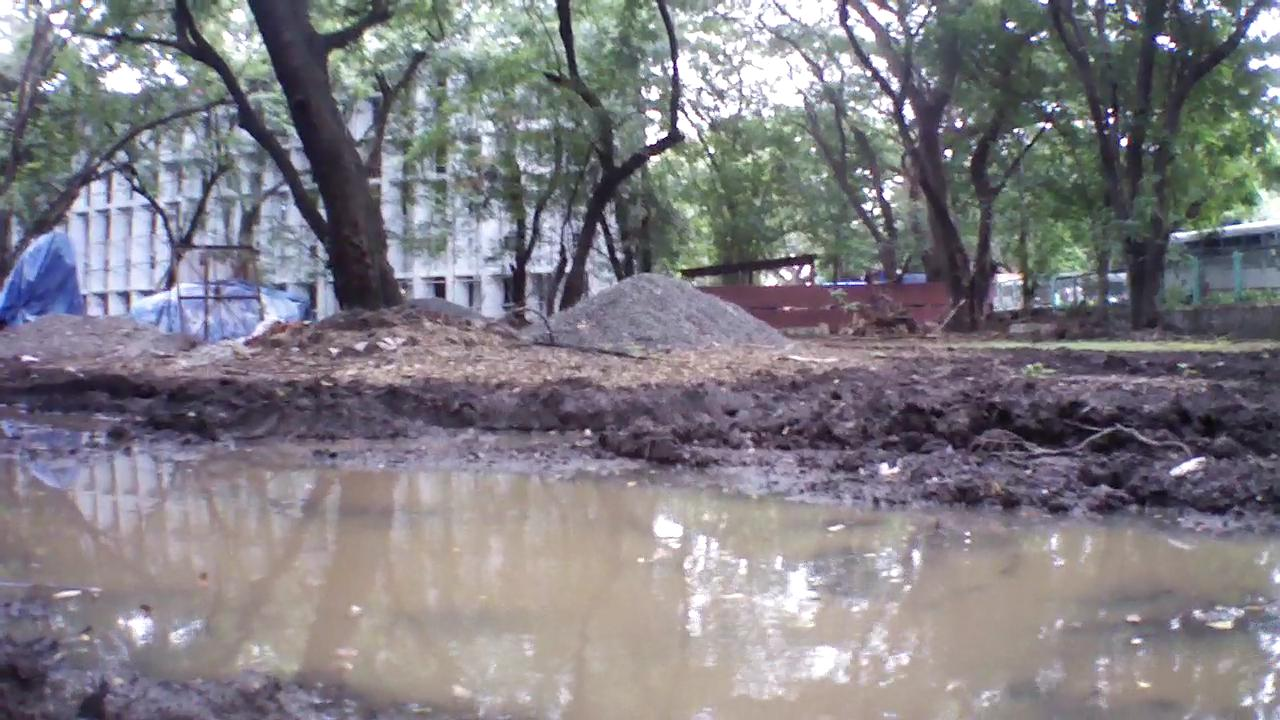
\includegraphics[width=0.32\linewidth]{stagnantWater/results/dataset_63full/IMG_PAIR_102_1} \hfill
  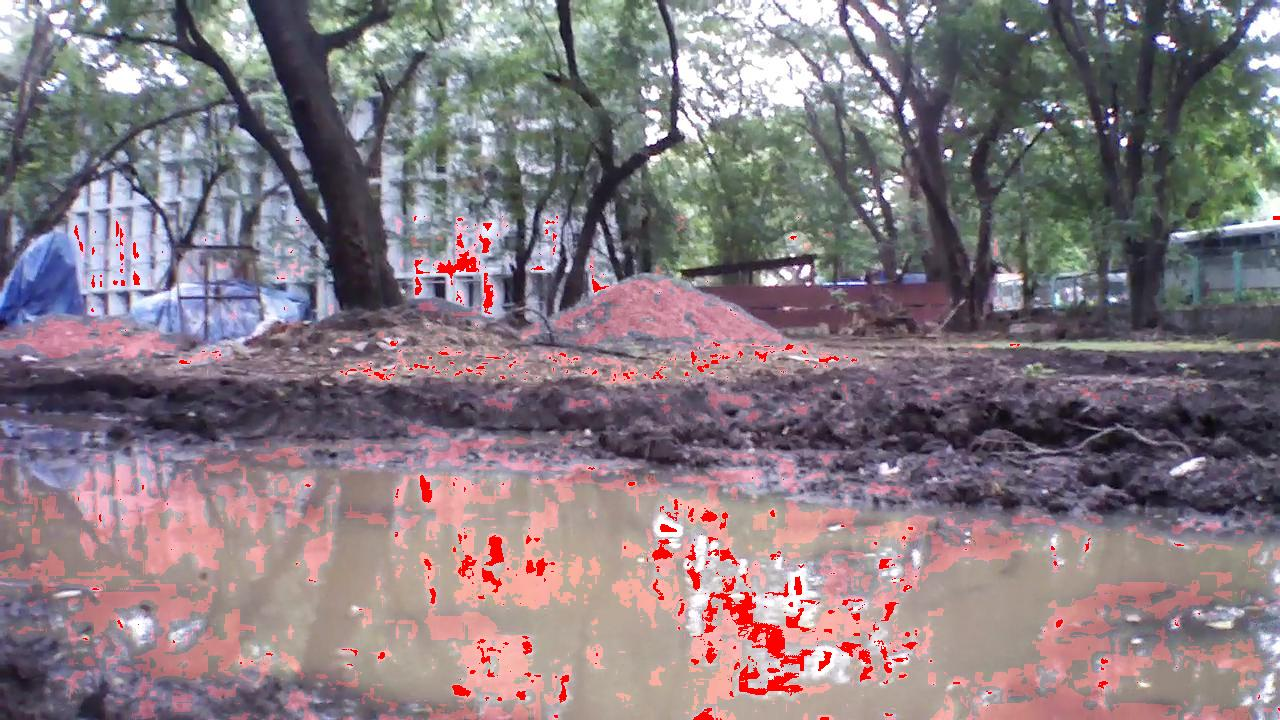
\includegraphics[width=0.32\linewidth]{stagnantWater/results/dataset_63full/output_102_jpl2} \hfill
  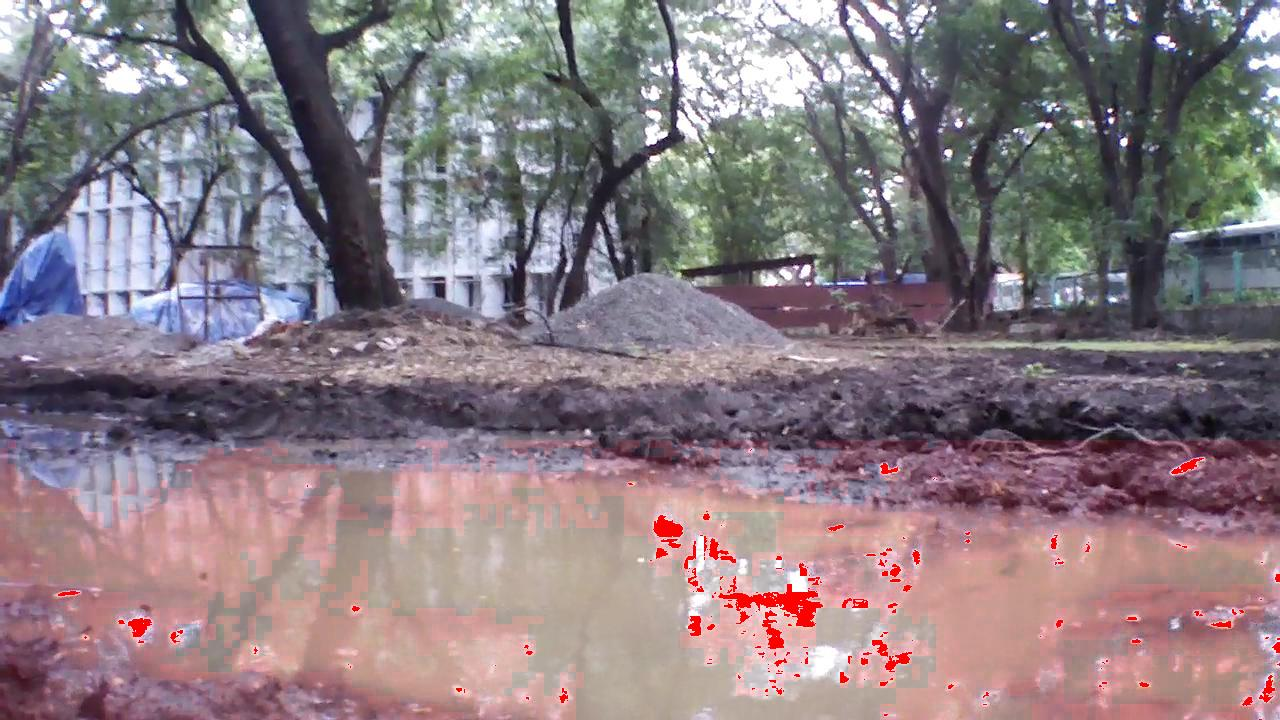
\includegraphics[width=0.32\linewidth]{stagnantWater/results/dataset_63full/output_102}
  	
  \caption{Comparison of proposed method with \cite{rankin2004daytime}. Confidence in detection is indicated by red hue in the output image. 
So, darker the red tinge, higher the confidence in detected water regions. \textbf{Left:} Original Image,
    \textbf{Middle:} Output of \cite{rankin2004daytime} \textbf{Right:}
    Proposed method. It can be seen that \cite{rankin2004daytime} is unable to
    detect textured puddle regions. Also, several false positives are
    seen to appear in the middle row.  Our method is sedate and
    sufficient to alert health workers.}
\label{fig:comparison}
\end{figure}

\newpage
\bibliographystyle{plain}
\bibliography{egbib}
\end{document}
